% !TeX spellcheck = fa_IR
% !TeX TS-program = xelatex
% Template based on IASBS Thesis, Version 2.40, Date: 2025/04/21
% بسته به اینکه مقصود شما رساله دکتری، پایان‌نامه ارشد یا پیشنهاد پروژه است یکی از خطوط زیر را فعال کنید.
% علاوه بر گزینه‌های زیر می‌توانید از سایر گزینه‌های سازگار با سبک report شامل 10pt، 11pt و غیره نیز استفاده کنید.
%\documentclass[a4paper,12pt,twoside,openright,phd,review]{iasbs-thesis}
\documentclass[a4paper,12pt,twoside,openright,phd]{iasbs-thesis}
%\documentclass[a4paper,12pt,twoside,openright,phd,proposal]{iasbs-thesis}
%\documentclass[a4paper,12pt,twoside,openright,master,review]{iasbs-thesis}
%\documentclass[a4paper,12pt,twoside,openright,master]{iasbs-thesis}
%\documentclass[a4paper,12pt,twoside,openright]{iasbs-thesis}

% اشکال و تصاویر هر فصل را در فولدر مربوطه کپی کنید. فایل‌ها در فولدرهای جدا هستند اما نباید همنام باشند. بنابراین از قالبی برای نامگذاری استفاده کنید که در آن شماره فصل مشخص باشد.
\graphicspath{{chap1_images/}{chap2_images/}{chap3_images/}{chap4_images/}{chap5_images/}}


% Prepare thesis information -------------------------------
% بسته به دانشکده، رشته، و گرایش یکی از موارد زیر را فعال کنید.
\department{Department of Physics}{دانشکدهٔ فیزیک}
\field{Physics}{فیزیک}
\subfield{Condensed Matter}{ماده چگال}
%\subfield{Complex Systems}{سامانه‌های پیچیده}
%\subfield{Soft Matter and Biological Physics}{مواد نرم و فیزیک زیستی}
%\subfield{Quantum Matter}{مواد کوانتومی}
%\subfield{Astronomy and Cosmology}{نجوم و کیهان‌شناسی}
%\subfield{Gravity}{گرانش}
%\subfield{Optics}{اپتیک}
%\subfield{Optics and Laser}{اپتیک و لیزر}
%\subfield{Optics and Photonics}{اپتیک و فوتونیک}
%
%\department{Department of Mathematics}{دانشکدهٔ ریاضی}
%\field{Mathematics}{ریاضیات}
%\subfield{Algebra}{جبر}
%\subfield{Financial Mathematics}{ریاضیات مالی}


\title{The Template of Theses}{
الگوی پایان‌نامه‌ها}
\subtitle{at the Institute for Advanced Studies in Basic Sciences}{
در دانشگاه تحصیلات تکمیلی علوم‌پایه زنجان}
%\subsubtitle{Subsubtitle of the Thesis}{دنبالهٔ عنوان طولانی}
\subsubtitle{Undergraduate Project Report, Master's Thesis, and Doctoral Dissertation}{
گزارش پروژهٔ کارشناسی، پایان‌نامه کارشناسی ارشد، و رسالهٔ دکتری}

% به صورت پیش‌فرض عنوان کوتاه که بالای صفحات زوج نمایش داده می‌شود معادل بخش اصلی عنوان است. اما اگر انتخاب دیگری دارید می‌توانید خط زیر را فعال کنید و عنوان کوتاه را تغییر دهید.
%\shorttitle{الگوی پایان‌نامه‌ها در دانشگاه}
\author{Name and Surname}{
نام و نام‌خانوادگی نویسنده}

% بسته به تعداد  اساتید راهنما و مشاور خطوط زیر را فعال یا غیرفعال کنید.
\supervisor{Name of First Supervisor}{
نام استاد راهنمای اول}
\supervisor{Name of Second Supervisor}{
نام استاد راهنمای دوم}
\advisor{Name of Advisor}{
نام استاد مشاور}
%\advisor{Name of Advisor}{نام استاد مشاور}

\date{\latintoday}{\today}
% تاریخ حقیقی برگزاری جلسه دفاع را با یکی از دو فرمت زیر وارد و جایگزین خط بالا کنید.
%\date{month day, year}{روز ماه سال}
%\date{month year}{ماه سال}


% درصورتی که مایلید پایان‌نامه خود را به شخصی که برایتان عزیز است تقدیم کنید، قسمت پیش‌رو را فعال کنید. در غیر این صورت این قسمت را غیر فعال کنید.
\dedication{
تقدیم به آنهایی که می‌خواهند بیشتر بدانند.
}
%اگر در فایل thanks.tex از دوستان، همکاران یا سایر اشخاص و منابعی که در پیشرفت پژوهش و پایان‌نامه شما نقش داشته اند تشکر کرده‌اید، خط زیر را فعال کنید، در غیر این صورت این خط باید غیرفعال باشد.
\acknowledgment{% !TeX root = main.tex
% !TeX spellcheck = fa_IR
در این بخش، بهتر است از افرادی که با کمک یا راهنمایی خود در پیشرفت پژوهش شما سهم داشته‌اند یا در نگارش و تصحیح پایان‌نامه به شما یاری رسانده‌اند، با ذکر دلیل قدردانی نمایید. این قدردانی می‌تواند بابت موارد زیر باشد:
\begin{enumerate}
\item 
استفاده از امکانات آزمایشگاهی یا محاسباتی خارج از گروه‌ پژوهشی استاد (اساتید) راهنمای شما،
\item
دسترسی و استفاده از داده‌ها یا نتایجی که دیگران در جمع‌آوری آن مشارکت داشته‌اند،
\item 
دسترسی به بانک نمونه‌های زیستی، معدنی و غیره که با تلاش سایر افراد جمع‌آوری شده است،
\item
استفاده از منابع و مخازن کد باز که توسط افرادی دیگر پیاده‌سازی شده‌اند،
\item 
استفاده از تصاویر، نمودارها، چارت‌ها یا هر سندی که قبلاً منتشر شده یا قبل از انتشار در اختیار شما قرار داده شده تا در پایان‌نامه شما درج شود و روند منطقی بیان موضوع را تکمیل کند.
\end{enumerate}
علاوه بر این‌ها، هر آنچه استاد (اساتید) راهنمای شما به شما یادآوری می‌کنند. ذکر منبع آنجا کفایت می‌کند که برای تایید و تکمیل بحث و نتیجه شما اضافه می‌شود. اما اگر چیزی را عیناً از منبع دیگری برمی‌دارید، علاوه بر اینکه این موضوع باید همانجا به صراحت ذکر شود، باید از صاحب اثر به نحو شایسته‌ای قدردانی شود. غیر از این‌ها شما ممکن است به سلیقه خود از کسانی که شما را در مسیر تحصیل و پژوهش حمایت کرده‌اند قدردانی کنید. فراموش نکنید ارزش این قدردانی به آن است که با واژه‌ها و جملات شما ابراز شود. سرقت ادبی حتی در متن این صفحه از ارزش کار شما می‌کاهد.

}


\abstract{% !TeX root = main.tex
% !TeX spellcheck = en_US
Sometimes, in journals, the abstract is limited to a short paragraph. Such a limitation makes writing abstracts for interdisciplinary research challenging. At the Institute for Advanced Studies in Basic Sciences (IASBS), there is no mandatory rule regarding the length of the abstract. However, keep in mind that the abstract should be the essence of your dissertation, and in many cases, achieving such a concise text requires effort and mastery over the content of the dissertation. Even the selection of keywords and their order needs meticulous attention. IASBS has entrusted the reviewers with the task of determining whether your effort has been sufficient.
}{% !TeX root = main.tex
% !TeX spellcheck = fa_IR
گاها در مجلات چکیده به یک پاراگراف کوتاه محدود می‌شود. چنین محدودیتی نگارش چکیده برای پژوهش‌های بین رشته‌ای را مشکل می‌کند. در دانشگاه تحصیلات تکمیلی علوم‌پایه زنجان قاعدهٔ لازم الاجرایی برای اندازهٔ چکیده وضع نشده است. اما در نظر داشته باشید که چکیده باید عصارهٔ
\thesis 
شما باشد و در بسیاری موارد، رسیدن به چنین متن خلاصه‌ای مستلزم تلاش و تسلط بر محتوی 
\thesis 
است. حتی انتخاب واژه‌های کلیدی و ترتیب آن‌ها نیاز به دقت و وسواس زیادی دارد. دانشگاه تشخیص اینکه تلاش شما کافی بوده را به داوران سپرده است.
}
\keywords{keyword 1, keyword 2, keyword3, ...}{
کلمه کلیدی ۱، کلمه کلیدی ۲، کلیمه کلیدی ۳، ...}

% خطوط زیر را متناسب با شرایط صفحه امضای کمیته داوری فعال یا غیرفعال و اصلاح کنید.
% به‌تناسب واژهٔ 'مرتبه` با یکی از موارد استادیار/دانشیار/استاد جایگزین شود.
% در صورت لزوم نام دانشکده یا دانشگاه را وارد یا تصحیح کنید.
% به تناسب قبل از نام‌ها از واژه دکتر/استاد استفاده کنید.
% اگر نام و نام خانوادگی اعضای کمیته طولانی است می‌توانید بخش میانی نام‌ها یا واژه‌های
% "Intenal/External/International"
% را به‌صورت
% "Intnl./Ext./Intl."
% مخفف بنویسید.
% Replace the term 'Rank' with one of the options: Assistant Professor, Associate Professor, or Professor.
% Enter or correct the name of the faculty or university if necessary.
% Use the titles Dr./Prof. before names as appropriate.
% If the full name of the committee members is lengthy, you may abbreviate the middle parts of the name or
% shorten the words "Internal/External/Interational" to "Intnl./Ext./Intl.".
\committeemember{Name and Surname}{Supervisor}{Rank, Department of Physics}{
نام و نام خانوادگی}{استاد راهنما}{مرتبه - دانشکدهٔ فیزیک}
\committeemember{Name and Surname}{Supervisor}{Rank, Department of Physics}{
نام و نام خانوادگی}{استاد راهنما}{مرتبه - دانشکدهٔ فیزیک}
\committeemember{Name and Surname}{Advisor}{Rank, Department of Physics}{
نام و نام خانوادگی}{مشاور}{مرتبه - دانشکدهٔ فیزیک}
\committeemember{Name and Surname}{Internal Reviewer}{Rank, Department of Physics}{
نام و نام خانوادگی}{داور داخلی}{مرتبه - دانشکدهٔ فیزیک}
\committeemember{Name and Surname}{Internal Reviewer}{Rank, Department of Physics}{
نام و نام خانوادگی}{داور داخلی}{مرتبه - دانشکدهٔ فیزیک}
%\committeemember{Name and Surname}{Internal Reviewer}{Rank, Department of Physics}{
%نام و نام خانوادگی}{داور داخلی}{مرتبه - دانشکدهٔ فیزیک}
\committeemember{Name and Surname}{External Reviewer}{Rank, University}{
نام و نام خانوادگی}{داور خارجی}{مرتبه - دانشگاه}
\committeemember{Name and Surname}{External Reviewer}{Rank, University}{
نام و نام خانوادگی}{داور خارجی}{مرتبه - دانشگاه}
%\committeemember{Name and Surname}{International Reviewer}{Rank, University}{
%نام و نام خانوادگی}{داور بین‌المللی}{مرتبه - دانشگاه}
\committeemember{Name and Surname}{Internal Reviewer \& Univ. Rep.}{Rank, Department of Physics}{
نام و نام خانوادگی}{داور داخلی و نماینده دانشگاه}{مرتبه - دانشکدهٔ فیزیک}
\committeemember{Name and Surname}{Univ. Rep.}{Rank, IASBS}{
نام و نام خانوادگی}{نماینده دانشگاه}{مرتبه - دانشکده}


\studentid{14xxyyzzzz}
\nationalid{0123456789}

%فهرست نماد‌ها برای پایان‌نامه‌هایی که تعداد زیادی کمیت با نمادهای مشابه در آن استفاده شده است ضروری است. برای مثال اگر در یک پایان‌نامه دو کمیت شتاب و اندازه سطح که نشانۀ کوتاه شده مشابهی برایشان انتخاب می‌شود به ترتیب با a و A نمایش داده شده باشند، وجود فهرستی برای مراجعه سریع به نمادها برای رفع ابهام ضروری خواهد بود. دقت کنید به هیچ وجه اجازه ندارید در طول یک پایان‌نامه دو کمیت متفاوت را با یک نشانۀ کوتاه شده یکسان بیاورید، ولو در دو فصل متفاوت. نمادها را می‌توانید ب دستور
%\addsymbolslist{symbol}{description}
%به فهرست نمادها اضافه کنید. اگر می‌خواهید فهرست نمادها دو ستونه شود خط زیر را فعال کنید.
%\twocolumnsybolslist

% نمونه‌ای از تعریف اصطلاحات پرتکرار برای تسهیل تایپ آنها در متن
%\newcommand{\dfa}{افت‌وخیز روندزدایی شده\xspace} % Example of chapter 3
%\newcommand{\kpz}{کاردر\dash پاریزی\dash ژانگ\xspace} % Example of chapter 3
%\newcommand{\md}{دینامول\xspace} % Example of chapter 3
% تعریف دستورات سفارشی برای لاتِک، زی‌لاتِک، و زی‌پرشین به فارسی با "ی" وارونه
\newcommand{\latex}{%
لا%
\hspace{-0.2em}ٰ\hspace{0.1em}%
تِک%
\xspace}
\newcommand{\xelatex}{ز%
\raisebox{0.5ex}{\reflectbox{ی}}\latex}
\newcommand{\xepersian}{ز%
\raisebox{0.5ex}{\reflectbox{ی}}%
پِرشــین%
\xspace}
%\usepackage{fontspec}
%\newcommand{\copyleft}{%
%    {\fontspec{FreeSerif}🄯} % Use a supplemental font for the copyleft symbol
%}

\initstyle % This must be the final command executed before the begin document.


\begin{document}

% Chapters of the Thesis -----------------------------------
% اگر مایل نیستید پیشگفتار داشته باشید می‌توانید خط بعدی را غیرفعال کنید. معمولاً برای پیشنهاد پروژه نیازی به پیشگفتار نیست.
% !TeX root = main.tex
% !TeX spellcheck = fa_IR
\section*{پیش‌گفتار}
\thispagestyle{plain} % Remove header on this specific page
\addcontentsline{toc}{section}{پیش‌گفتار}
الگوی قدیمی صفحه‌آرایی و حروف‌چینی رساله‌ها و پایان‌نامه‌ها براساس امکاناتی نظیر ماشین‌تحریر شکل گرفته بود. به همین سبب، لازم بود صفحات در قطع 
$\mathrm{A4}$، 
یک خط در میان، و یک‌رو حروفچینی شوند و با جلدی ضخیم صحافی شوند تا نگهداری آن‌ها برای مدت طولانی ممکن باشد. با رشد روزافزون فناوری، سال‌هاست که در بسیاری از دانشگاه‌های دنیا این الگوی قدیمی کنار گذاشته شده است و پایان‌نامه‌ها به مدد امکانات رایانه‌ای و چاپگرهای لیزری با طرحی شبیه کتاب آماده و تدوین می‌شوند.

به همین سبب از مدتی قبل لزوم تدوین و انتشار الگویی که بر پایهٔ فناوری روز بنا شده باشد احساس می‌شد و شورای آموزش دانشگاه تحصیلات تکمیلی علوم‌پایه زنجان نیز با تصویب یک مصوبه و ارائه یک راهنما این نیاز را تایید کرد. الگوی حاضر برمبنای همان راهنما و با مشورت جمعی از اساتید دانشکدهٔ فیزیک تدوین شده است. تلاش شده تا حد ممکن نکات ظریف بیان شده در آن راهنما در این الگو گنجانده شود. با این وجود توصیه می‌شود قبل از شروع به نگارش 
\thesis 
و اعمال تغییرات در محتوی این الگو، حتماً یکبار آن راهنما را مطالعه کنید.

الگوی حاضر برمبنای کلاس\dash سند 
\lr{`iasbs-thesis.cls'} 
طراحی شده است. در این کلاس علاوه بر گزینه‌های شناخته شدهٔ کلاس\dash سند
\lr{`report'} 
در لاتک می‌توانید از گزینه‌های 
\lr{`phd'}، \lr{`master'}، \lr{`proposal'}، \lr{`review'}، 
نیز استفاده کنید. با ترکیب مناسب این گزینه‌ها می‌توان از این الگو برای نگارش نسخهٔ نهایی، پیش‌نویس، یا پیشنهادِ رسالهٔ دکتری و یاپایان‌نامهٔ کارشناسی ارشد استفاده کرد. در صورت تمایل حتی می‌توانید پروژه کارشناسی را نیز با آن بنویسید. بسته به انتخاب شما و ترکیب گزینه‌های کلاس، عملکرد کلاس تغییر می‌کند و چیدمان، تعداد صفحات ابتدا و انتهایی را تنظیم می‌کند. حالت پیش‌نویس برای تسهیل مرور متن 
\thesis 
برای اساتید راهنما، مشاور و داوران ترتیب صفحات را تغییر می‌دهد و صفحات متناظر فارسی و انگلیسی را پشت سر هم قرار می‌دهد تا مقایسه و تطبیق آنها ساده شود. با حذف این گزینه، ترتیب درست صفحات انتخاب می‌شود. صفحاتی مثل قدردانی و حق تألیف در پیشنهاد پروژه حذف می‌شوند. برای روشن شدن موضوع و همینطور به‌قصد آموزش نحوهٔ ساخت جداول بزرگ در فصل روش‌ها جدولی گنجانده شده است که چیدمان صفحات را براساس گزینه‌های انتخابی نشان می‌دهد، جدول~
\ref{tab3:3}.

این الگو به‌طور پیش‌فرض برای چاپ روی کاغذ 
\lr{A4} 
آماده شده است. این حالت برای پیش‌نویس و پیشنهاد
\thesis 
مناسب است. با این حال برای نسخهٔ نهایی 
\thesis 
می‌توانید آن را در کاغذ 
\lr{B5 
(با ابعاد 
$177\unit{mm} \times 249\unit{mm}$}) 
چاپ کنید. برای این کار، بسته به قابلیت‌های چاپگر، می‌توانید صفحات را در مقیاس 
$84\,\%$ 
چاپ کنید یا حاشیه‌های چپ و راست کاغذ 
\lr{A4} 
را از هر طرف 
$16.5\unit{mm}$ 
و حاشیه‌های بالا و پایین را 
$24\unit{mm}$ 
کوچک کنید. پس از صفحات اصلی 
\thesis 
دو صفحهٔ اضافی چاپ می‌شود که در شمارش صفحات لحاظ نمی‌شوند. صفحهٔ اول خطوط برش را برای کاغذ 
\lr{A4} 
نشان می‌دهد تا برش صفحات به اندازهٔ 
\lr{B5} 
ساده شود. صفحه بعد، که آخرین صفحهٔ اضافی است، جلد است. این صفحه باید در کاغذ گلاسه با ابعاد 
\lr{A3} 
(با اندازهٔ 
$297\unit{mm} \times 420\unit{mm}$) 
چاپ شود و سپس از روی خطوط راهنما برش بخورد تا جلد مناسب نسخهٔ
\lr{B5} 
به‌دست آید. لازم به ذکر است که ضخامت شیرازه براساس کاغذ $80$ گرمی محاسبه می‌شود. عمداً صفحه جلد از طرفین دو میلیمتر بزرگ‌تر در نظر گرفته شده است تا تطبیق لبه‌های صفحات با جلد در برش نهایی ساده‌تر انجام شود.


\subsubsection{علت نگارش پیش‌گفتار}
در شرایط عادی اگر فصل مقدمه را خوب بنویسید نیازی به نگارش پیشگفتار ندارید و می‌توانید آن را حذف کنید. اما خصوصاً در موضوعات بین رشته‌ای یا وقتی پژوهش شما شامل بخش‌های متنوع تئوری، تجربی و محاسباتی است، ساختار 
\thesis 
ممکن است پیچیده‌تر از حالت معمول باشد. در این موارد، حتی ممکن است مجبور شوید بیش از یک فصل مقدمه داشته باشید. در چنین شرایطی بهتر است پیشگفتار نوشته شود. 

در پیشگفتار می‌توانید مفصل‌تر از چکیده، مسأله را شرح دهید و علت ساختار پیچیده 
\thesis 
را روشن کنید. در فصول بعدی شما نمی‌توانید قبل از بیان یک مفهوم از آن استفاده کنید و ملزم به رعایت سیر منطقی هستید. بنابراین ممکن است بحث‌های مفصل و گسترده‌ای لازم باشد تا مقدمات بیان مسأله فراهم شود. در پیشگفتار لازم نیست مسأله به‌طور دقیق بیان شود، به همین دلیل نیاز به مقدمه‌چینی کمتری است. از طرفی، با طرح مساله در پیشگفتار، می‌توان مسیر و ساختار 
\thesis 
را بهتر بیان کرد و ذهن خواننده را برای دنبال کردن مقدمات آماده و توجیه کرد.

در اینجا لازم می‌دانم از تمامی دوستان و همکارانی که با مطالعه متن الگوی حاضر در رفع ایرادها و تکمیل آن مشارکت کردند، تا الگویی مناسب برای دانشجویان فراهم شود، تقدیر و تشکر کنم. همچنین سپاسگزار خواهم شد که پیشنهادات و مشکلات این الگو را که ضمن استفاده از آن  مشخص خواهد شد با ایمیل%
\LTRfootnote{\href{mailto:m.d.niry@iasbs.ac.ir}{m.d.niry@iasbs.ac.ir}} 
برایم ارسال فرمایید.\\[1em]
محمّد دهقان نیری\\
هیات علمی دانشــکده فیزیک\\
زمسـتان ۱۴۰۳

             % پیشگفتار
% !TeX root = main.tex
% !TeX spellcheck = fa_IR
\chapter{مقدمه}
در نگارش این الگو تعمداً سعی شده است علاوه بر ارائه توضیحات آموزشی از ابزار‌های مختلف 
\xepersian 
و 
\latex 
استفاده شود. شما می‌توانید این موارد را به عنوان مثال ببینید و استفاده کنید. 

معمولا ساختار \thesis به چند فصل تقسیم می‌شود. محتوی و نام‌گذاری این فصول سلیقه‌ای است. یکی از انتخاب‌ها به شرح زیر است،
\begin{enumerate}
\item
مقدمه، 
\item 
تاریخچه، 
\item 
مواد و روش‌ها (الگوریتم‌ها و روش‌ها)، 
\item 
نتایج، 
\item 
بحث و جمع‌بندی.
\end{enumerate}
شما می‌توانید تاریخچه را به‌طور مختصر در مقدمه بیان کنید و فصل تاریخچه را حذف کنید. کافیست خط
\begin{latin}\begin{verbatim}
% !TeX root = main.tex
% !TeX spellcheck = fa_IR
\chapter{تاریخچه پژوهش}

در این بخش به معرفی کلی پژوهش‌های انجام شده در زمینه مورد نظر پرداخته می‌شود. هدف اصلی این فصل، ارائه تصویری جامع از پیشینه مسأله و پژوهش است. ممکن است به جای این فصل قسمتی از مقدمه به بیان تاریخچه مسأله اختصاص یابد و این فصل حذف شود.

این فصل می‌تواند با بررسی کارهای مرتبط پژوهشی که در گروه پژوهشی که در آن عضویت دارید آغاز شود. سپس به بررسی پژوهش‌های مرتبط که داخل کشور انجام شده بپردازید و نهایتا با مرور مسأله‌های مرتبط که در مقالات گروه‌های بین‌المللی گزارش شده خاتمه یابد.

میزان شرح و بسط تاریخچه تا حدی به سلیقه شما و موضوع و مسأله‌ای که روی آن کار می‌کنید بستگی دارد. استاد راهنما می‌تواند در این مورد بهترین راهنمایی را به شما بدهد.

\section{جمع‌بندی}
در این قسمت، نتایج مرور پژوهش‌های انجام شده خلاصه و تحلیل می‌شوند. این تحلیل می‌تواند به شناسایی نقاط قوت و ضعف تحقیقات قبلی و تعیین شکاف‌های پژوهشی که قرار است پروژه پژوهشی شما برخی از آنها را پر کند، کمک کند.


\end{verbatim}
\end{latin}\noindent
را در 
\lr{main.tex}
غیرفعال کنید تا فصل تاریخچه حذف شود. ممکن است بسته به موضوع، ترتیب فصول تغییر داده شود یا فصول جدیدی اضافه شود. در انجام این کار با هدایت استاد راهنما آزاد هستید. هدف نگارش 
\thesis 
به‌نحوی است که برای خواننده درک و دنبال کردن آن ساده‌تر باشد. در واقع، مهمترین هدف از نگارش هر متن علمی انتقال حداکثر مفاهیم است. 

در هر فصل، یک قالب پیشنهادی برای بخش‌بندی فصل ارائه شده است که کاملاً سلیقه‌ای است و شما در تغییر آن بسته به موضوع و مسأله خود کاملاً آزاد هستید. علاوه بر آن در فصل روش‌ها نحوه نگارش 
\thesis 
و استفاده از 
\latex 
برای ایجاد شکل و جدول توضیح داده شده است. 

در ادامه ساختار پیشنهادی فصل مقدمه را می‌آوریم. مقدمهٔ 
\thesis
باید به سوالاتی پاسخ دهد. لازم نیست حتماً جواب هر سوال در یک بخش داده شود. ممکن است جواب برخی از این سوالات را در یک پاراگراف بیاورید. بنابراین می‌توانید این بخش‌بندی را به سلیقه خودتان تغییر دهید و بعضی موارد را با هم ترکیب کنید. هدف این است که سوالاتی که قرار است در مقدمه به آنها پاسخ دهید یکجا یادآوری شوند:


\section{زمینه و اهمیت موضوع}
مقدمه می‌بایست زمینهٔ پژوهش را توضیح دهد و اهمیت و ارزش موضوع پژوهش را به وضوح بیان کند. چرا این مسأله مهم است و حل آن چه تاثیری می‌تواند در حوزهٔ علمی مورد نظر داشته باشد؟


\section{مسألهٔ پژوهش}
در هر پژوهشی مسألهٔ می‌بایست به‌طور دقیق و واضح تعریف شود. بهترین نقطه برای انجام این کار مقدمه است. باید مشکل یا چالشی که قصد دارید در این پژوهش حل کنید را بیان کنید. ممکن است در ابتدای مقدمه نتوانید تعریف دقیق مسأله را بیان کنید. اما بعد از بیان مفاهیم می‌توانید مسأله را به‌صورت دقیق بیان کنید.


\section{اهداف پژوهش}
اهداف کلی و جزئی پژوهش خود را مشخص کنید. اهداف باید واقع‌بینانه، قابل دستیابی و مرتبط با مسألهٔ باشند. این قسمت به‌نحوی با بیان مسأله مرتبط است و ممکن است بخواهید هر دو را در قالب یک بخش بیان کنید.


\section{سوالات یا فرضیات پژوهش}
در این قسمت، دانشجو باید سوالات اصلی و فرعی یا فرضیات را مطرح کند. این سوالات یا فرضیات باید به گونه‌ای باشند که بتوان آن‌ها را در طول پژوهش پاسخ داد یا آزمایش کرد.


\section{ساختار رساله/پایان‌نامه}
اگر از قالب شناخته شده فصل‌بندی استفاده نمی‌کنید حتما باید به‌طور مختصر به ساختار کلی 
\thesis 
اشاره کنید و توضیح دهد که هر فصل شامل چه مباحثی می‌باشد. اما ممکن است ترجیح دهید این کار را در پیشگفتار انجام دهید.


\section{محدودیت‌های پژوهش}
با مطالعه تاریخچه مسأله متوجه محدودیت‌ها و چالش‌هایی می‌شوید که در حل مسأله با آن‌ها مواجه خواهید شد. می‌توانید به چنین مواردی در فصل مقدمه یا بسته به مورد در فصل تاریخچه اشاره کنید.


\section{تعریف اصطلاحات}
حل هر مسأله به شناخت مفاهیمی متکی است که ممکن است جزء دانش عمومی خوانندگان نباشد. مقدمه حتماً باید شامل بخشی باشد که اصطلاحات کلیدی مورد استفاده در پژوهش را تعریف کند تا خواننده با مفاهیم مورد بحث آشنا شود.

رعایت این ساختار الزامی نیست، اما با بیان همه موارد ذکر شده، مقدمه‌ای جامع و کامل برای 
\thesis 
تهیه می‌شود که به خواننده کمک می‌کند تا با زمینهٔ پژوهش، اهمیت آن، اهداف و سوالات مطرح، و ساختار کلی 
\thesis
آشنا شود.
           % مقدمه
% اگر تاریخچه را به عنوان بخشی از مقدمه نوشته‌اید می‌توانید خط بعدی را غیرفعال کنید.
% !TeX root = main.tex
% !TeX spellcheck = fa_IR
\chapter{تاریخچه پژوهش}

در این بخش به معرفی کلی پژوهش‌های انجام شده در زمینه مورد نظر پرداخته می‌شود. هدف اصلی این فصل، ارائه تصویری جامع از پیشینه مسأله و پژوهش است. ممکن است به جای این فصل قسمتی از مقدمه به بیان تاریخچه مسأله اختصاص یابد و این فصل حذف شود.

این فصل می‌تواند با بررسی کارهای مرتبط پژوهشی که در گروه پژوهشی که در آن عضویت دارید آغاز شود. سپس به بررسی پژوهش‌های مرتبط که داخل کشور انجام شده بپردازید و نهایتا با مرور مسأله‌های مرتبط که در مقالات گروه‌های بین‌المللی گزارش شده خاتمه یابد.

میزان شرح و بسط تاریخچه تا حدی به سلیقه شما و موضوع و مسأله‌ای که روی آن کار می‌کنید بستگی دارد. استاد راهنما می‌تواند در این مورد بهترین راهنمایی را به شما بدهد.

\section{جمع‌بندی}
در این قسمت، نتایج مرور پژوهش‌های انجام شده خلاصه و تحلیل می‌شوند. این تحلیل می‌تواند به شناسایی نقاط قوت و ضعف تحقیقات قبلی و تعیین شکاف‌های پژوهشی که قرار است پروژه پژوهشی شما برخی از آنها را پر کند، کمک کند.

           % تاریخچه
% !TeX root = main.tex
% !TeX spellcheck = fa_IR
%\chapter{مواد و روش‌ها} % برای پژوهش‌های تجربی یا
%\chapter{الگوریتم‌ها  و روش‌ها} % الگوریتم‌ها و روش‌ها در پژوهش‌های عددی
\chapter{روش‌ها}
اگر پروژه شما تجربی باشد، در این فصل به معرفی کلی مواد و روش‌های استفاده شده پرداخته می‌شود. این بخش باید به گونه‌ای نوشته شود که خواننده بتواند روند کلی پژوهش را درک کند. در ادامه، احتمالاً بخشی به مواد اختصاص می‌یابد که در آن فهرستی از مواد اولیه مورد استفاده (شامل مواد شیمیایی، نمونه‌ها، غیره) و ویژگی‌های آنها ذکر می‌شود. سپس ابزارهای مورد نیاز فهرست می‌شوند و بخش بعدی به روش آماده‌سازی مواد، روش‌های آزمایش و تحلیلی نتایج  اختصاص می‌یابد. نهایتا بخشی نیز به جمع‌بندی مطالب این فصل اختصاص می‌یابد.

اگر پروژه شما محاسبات عددی یا شبیه‌سازی باشد، ترتیب مطالب این فصل تفاوت چندانی ندارد. فقط به‌جای مواد و ابزارها از روش‌ها و الگوریتم‌ها صحبت خواهید کرد و ویژگی‌ها و تفاوت‌های آنها را بیان خواهید کرد. باز هم باید مطالبی در مورد تحلیل نتایج و داده‌ها داشته باشید و سرآخر جمع‌بندی خواهید داشت.

در ادامه این فصل به بیان روش نگارش پایان‌نامه یا رساله با استفاده از سیستم حروف‌چینی 
\xelatex\LTRfootnote{\XeLaTeX} 
و زیرمجموعهٔ آن بستهٔ 
\xepersian\LTRfootnote{\XePersian} 
می‌پردازیم. توضیحات و راهنمایی‌ها با نمونه و مثال ارائه می‌شوند تا کار نگارش اصطلاحات علمی، عبارت‌ها و روابط ریاضی، شکل‌ها و جداول را برایتان ساده کنند. 

مهمترین کاری که باید بتوانید انجام دهید، ارجاع درست به پژوهش‌های پیشین است. این مراجع ممکن است مقاله 
\cite{myers2013improving}، 
کتاب 
\cite{willey2008prescott}، 
پایان‌نامه کارشناسی ارشد 
\cite{Iri}، 
رسالهٔ دکتری 
\cite{Mostafavi}، 
یا صفحات تارنما%
\LTRfootnote{webpages} 
باشند 
\cite{thesis}. 
شیوه ارجاع در متن به همهٔ آنها یکسان است، اما قالب هریک تفاوت‌های کوچکی دارد. اینجا از هریک مثالی آورده‌ایم تا شما بتوانید با مراجعه به فایل 
\lr{`MyReferences.bib'} 
تفاوت‌ها را ببینید. این روزها دانشجویان فراوان به دانشنامه‌های آنلاین نظیر دانشنامهٔ آزاد ویکی‌پدیا ارجاع می‌دهند. در این موارد فراموش نکنید که از لینک دائمی به صفحه استفاده کنید تا تغییرات زمانی صفحات آنلاین مرجع شما را مخدوش نکند.

برای نگارش 
\thesis 
ممکن است مفاهیم و کمیت‌هایی را از منابع دیگر یادبگیرید و به‌کارگیرید. ممکن است در مستندات علمی نمادها و نشانه‌های متفاوتی برای این کمیت‌ها متداول باشد و منبعی که از آن استفاده می‌کنید، یکی از آنها را به‌کار گرفته باشد. شما اجازه ندارید به دو کمیت یا مفهوم متفاوت یک نماد اختصاص دهید، بنابراین لازم است متناسب با کمیت‌ها و مفاهیم به‌کار رفته در نوشتارتان و میزان تکرار هر مفهوم الگوی سازگاری از نمادها را به کمیت‌ها اختصاص دهید که یکتا و با مسما باشد. فهرست نمادها می‌تواند در انتخاب نمادهای غیر تکراری به شما کمک کند. برای مثال $w$ برای نشان دادن پهنا، وزن و کار استفاده می‌شود. از هر سه کمیت نیاز باشد، می‌توان پهنا را با $w$ نشان داد، وزن را با $W$ و کار را با
$\mathcal{W}$. 
به این ترتیب با حفظ سازگاری همه کمیت‌ها قابل تشخیص خواهند بود. این کمیت‌ها را می‌توان به فهرست نمادها نیز اضافه کرد.
\addsymbolslist{$w$}{پهنا}
\addsymbolslist{$W$}{وزن}
\addsymbolslist{$\mathcal{W}$}{کار}

به مرور که در متن با نمادهای جدید روبرو می‌شوید، آنها به فهرست اضافه کنید. به این ترتیب می‌توانید با مرور فهرست نمادهای بعدی را راحت‌تر انتخاب کنید. 
اگر تعداد نمادها در 
\thesis 
شما خیلی زیاد است و از طرفی تعریف آنها طولانی نیست، می‌توانید با دستور 
$\backslash\texttt{twocolumnsymbolslist}$ 
فهرست نمادها را دو ستونه کنید، زیرا فضای خالی سمت چپ صفحات فهرست زیبا به نظر نمی‌رسد.

\normalfootnotes
معمولاً از زیرنویس برای معرفی معادل انگلیسی اصطلاحات و واژه‌های جدید و همچنین نام پژوهشگران استفاده می‌کنیم. به همین دلیل بیشتر زیرنویس‌ها تنها به اندازهٔ یک واژه طول دارند. اگر تعداد زیرنویس‌ها در یک صفحه زیاد باشد، چند سطر خالی در پایین صفحه ظاهر می‌شود که زیبا نیست. در پاورقی‌ها این الگو معادل انگلیسی واژه‌ها در دو ستون مرتب شده است تا فضای خالی در پایین صفحات ایجاد نشود. اما گاهاً ناچاریم یک توضیح یا تعریف نا مرتبط با سیر منطقی بحث را برای خواننده در پاورقی بیاوریم. چنین توضیحاتی در نیم خط نمی‌گنجند%
\footnote{
وقتی می‌خواهیم یک زیرنویس طولانی چند خطی داشته باشیم. بهتر است، موقتاً زیرنویس‌ها را یک ستونه کنیم و بعد دوباره آنها را به حالت دو ستونه برگردانیم. در اینجا عمداً این توضیح را در پاورقی آوردیم، تا به‌عنوان یک نمونه قابل استفاده باشد.}.
\twocolumnfootnotes

لزومی ندارد تمام این فصل را کامل مطالعه کنید. ابتدا روش‌های ساده را یاد بگیرید و کار نگارش 
\thesis  
را شروع کنید. هر زمان با مشکلی مواجه شدید، می‌توانید به محتوی این فصل نگاهی بیاندازید و از مثال‌های آن استفاده کنید.


\section{قواعدی ساده در نگارش متن}
در گذشته زمانی که حروف‌چینی و چاپ آغاز شد برای کاهش هزینه‌ها افراد ناوارد کار حروف‌چینی را انجام می‌دادند. همین مسأله سبب شد، همزه و 'ی` نکره که بعد از 'ـه` آخر می‌آمد با حروف یکسان حروف‌چینی شود. بعدها برای آگاهی عموم فارسی‌زبان‌ها پیشنهاد شد که 'ی` نکره به صورت کامل نوشته شود، مثلاً بنویسیم 'مسأله‌ی` یا 'معادله‌ی`. بعد از مدتی متوجه شدیم در گذشته‌های دور وقتی هنرمندان خطاط می‌خواستند 'ی` نکره را بنویسند، آن را خیلی کوچک بالای 'ـه` آخر می‌گذاشتند.  به همین سبب، امروزه نیز توصیه می‌شود، اگر محیط نگارش اجازه می‌دهد، به رویه گذشته عمل کنیم. خوشبختانه نسخه‌های اخیر بستهٔ حروف‌چینی 'بای‌دی`%
\LTRfootnote{\textsf{bidi} (bidirectional typesetting)}
که 
\xepersian 
از آن بهره می‌برد، به شرط نصب قلم‌های استاندارد فارسی، این قابلیت را دارد. بنابراین بهتر است به‌جای مسأله‌ی بنویسیم "مسألهٔ``. به تفاوت علامت همزه (ء) و 'ی` کوچک در این واژه دقت کنید.

در نگارش متن فارسی، رایج است که کلمات مرکب، پیشوندها و پسوندها با نیم‌فاصله نوشته شوند. نیم‌فاصله یا به عبارت درست‌تر فاصله مجازی%
\LTRfootnote{Zero-width non-joiner (ZWNJ)} 
در جانمایی‌های%
\LTRfootnote{keyboard layouts} 
مختلف صفحه‌کلید با ترکیب متفاوتی از کلیدها تایپ می‌شود، مثلاً:
\lr{Shift+Space}، \lr{Ctrl+Shift+2}، \lr{Shift+b}، یا \lr{Alt+0157}. 
در آخرین مورد، اعداد را باید با صفحه‌کلید عددی%
\LTRfootnote{numpad} 
تایپ کنید. اگر هیچ یک از این ترکیبات برای شما کار نمی‌کند، خودتان می‌توانید برای آن یک میانبر تعریف کنید. 

در نگارش برخی کلمات مرکب مثل اسامی خاص، بهتر است از خط تیره (-) به‌جای نیم‌فاصله استفاده شود. مثلاً بهتر است بنویسیم مدل کاردر\dash پاریزی\dash ژانگ%
\LTRfootnote{Kardar-Parisi-Zhang}. 
این علامت را با خط تیره طویل (--) که برای نشان دادن یک بازه استفاده می‌شود اشتباه نگیرید، مثلاً سال‌های ۱۳۶۸--۱۳۵۸. خط تیره بسیار طولانی (---) هم برای مشخص کردن جملات معترضه استفاده می‌شود. مثلاً، دقت در انجام پژوهش ---گرچه زحمت زیادی دارد--- به نتایج افتخار آمیز منجر می‌شود. در فارسی خط کرسی نیز هست که برای کشــــــیده نوشتن کلمات استفاده می‌شود.

گاهی احتیاج خواهید داشت که از گیومه برای نقل قول یا برجسته کردن یک واژه استفاده کنید. انتخاب الگوی "انگلیسی`` یا «فرانسوی» به سلیقه شما بستگی دارد، اما بهتر است از الگوی یکسانی برای تمام متن استفاده کنید. گیومه را می‌توان 'یگانه` یا "دوگانه`` گذاشت. به جهت چرخش و تفاوت نماد گیومه در دو طرف واژه توجه کنید. این ظرافت‌ها اگرچه در مفهوم مطلبی که می‌نویسید بی‌اثر است، اما توجه و وسواس شما خواننده را از دقت و مهارت شما در انجام پژوهشی که به آن پرداخته‌اید، مطمئن می‌سازد. یک راه ساده‌تر برای برجسته کردن بخشی از متن 
\emph{ایرانیک} 
نوشتن آن است.

اصلی‌ترین دلیل استفاده از گیومه نقل قول است. ما معمولاً مفاهیم و روابط را با زبان خودمان بیان می‌کنیم و تنها برای جزئیات و سندیت موضوع به دیگران ارجاع می‌دهیم. اما ممکن است برای نشان دادن اهمیت یک موضوع، بیان فرد دیگری را عیناً به عاریت بگیریم. مثلاً، در ابتدای مقدمه یک
\thesis 
در زمینه تلاطم برای رساندن اهمیت و پیچیدگی مسأله، چند جمله‌ای منتسب به وِرنر هایزنبرگ%
\LTRfootnote{Werner Heisenberg} 
را نقل کنیم تا خواننده را به هیجان آوریم. این چند جمله می‌تواند به زبان انگلیسی باشد:
\lr{\begin{quote}
``When I meet God, I am going to ask him two questions: Why relativity? And why turbulence? I really believe he will have an answer for the first." \cite{Wiscombe2005}
\end{quote}}
یا به فارسی ترجمه شده باشد:
\begin{quote}
«وقتی خداوند را ملاقات کنم، دو سوال از او خواهم پرسید: چرا نسبیت؟ و چرا تلاطم؟ واقعاً باور دارم که او برای اولین سوال پاسخ خواهد داشت.» 
\cite{Wiscombe2005}
\end{quote}
این‌که کدام را ترجیح دهیم به متن نقل قول و خواننده هدف بستگی دارد و اندکی سلیقه‌ای است. حتی ممکن است، یکی را در متن اصلی و دیگری را در پاورقی بیاوریم. مهم این است که متن نقل قول در گیومه و در محیط 
\lr{``quote"} 
آورده شود تا پهنای آن نسبت به متن اصلی کاهش یابد و به وضوح از متن 
\thesis 
متفاوت و قابل تشخیص و تفکیک باشد.


\section{نگارش روابط ریاضی}
در این الگو برای نگارش اعداد از قلم 'یاس` استفاده می‌کنیم، زیرا صفر آن توخالی است. برای مثال عدد 
$100$
را ببینید. برای مقادیر عددی دارای واحد نظیر،
$30.2\unit{mm}$ 
یا
$T_\mathrm{r} = 24\unit{\degC}$
می‌توانید از دستور ساده 
$\backslash\mathrm{unit}\{\mbox{\small\rl{واحد}}\}$ 
استفاده کنید. دقت کنید که در محیط فرمول پارامترها 
\textit{ایتالیک} 
نوشته می‌شوند. اما هرچیز مخفف یک کلمه باشد، بایستی به‌صورت طبیعی رومی%
\LTRfootnote{roman} 
نوشته شود. مثلاً واحدها (میلی‌متر، سانتیگراد و جز این‌ها)، نام توابع ریاضی (سینوس، کسینوس، و غیره)، یا نام عناصر شیمیایی را 
\textit{ایتالیک}  
نمی‌نویسیم،
\begin{equation*}
\mathrm{H}_2 + \tfrac{1}{2}\mathrm{O}_2 \longrightarrow \mathrm{H_2O}.
\end{equation*}

برای تبدیل فوریه تابع 
$f(x)$، 
می‌توان نوشت
$\mathcal{F}[f(x)]$.
این نمونه‌ای از یک رابطهٔ ریاضی داخل متن است. سعی کنید در متن، عبارات ریاضی را تا حد ممکن بدون توان و خط کسری بنویسید تا فاصله خطوط متن یکنواخت بماند و قلم عبارت‌های ریاضی نیز خیلی ظریف نشود. مثلاً به‌جای 
$L^{-1}$ یا $\frac{1}{L}$ 
در متن بنویسید، 
$1/L$.

ممکن است بخواهیم یک رابطه را در یک خط جدا بنویسیم. مثلاً،
\begin{equation}\label{eq1:1}
f(r) = \int_0^r \int_0^\pi r\sin\theta \d r \d\theta,
\end{equation}
یا برخلاف رابطهٔ~
\eqref{eq1:1} 
بخواهیم تعریف ماتریس پاولی را بدون شماره بیاوریم،
\begin{equation*}
\sigma_1 = \left(\begin{array}{ll}
0 & 1\\
1 & 0
\end{array}\right).
\end{equation*}
علامت '$*$` در کنار نام محیط 
\lr{`equation'} 
سبب شده، رابطه شماره نخورد. می‌توان یک رابطهٔ گسسته را هم نوشت، مثلاً 
$\sum_{i=1}^{n}x_i$.

در ادامه به عنوان نمونه دیگر، یک رابطهٔ سه‌خطی می‌آوریم،
\begin{eqnarray}\label{eq1:2}
h(x) &=& \int x^2\left(1+x^2\right) \d x\nonumber\\
&=& \tfrac{1}{3} x^3 + \tfrac{1}{5} x^5 + C,\\
q(x) &=& \frac{1}{1+\exp(-\beta x)}.\label{eq1:3}
\end{eqnarray}
دستور  
$\backslash\texttt{nonumber}$ 
سبب شد، خط اول رابطهٔ~%
\eqref{eq1:2} 
شماره نخورد. به ردیف شدن علامت‌های تساوی در سه‌خط رابطه توجه کنید. این نتیجه درج علامت‌های تساوی میان دو علامت 
'$\&$` 
است. همچنین ببینید که چگونه اندازه پرانتزها در خط اول با محتوی هماهنگ گشته است. این نتیجهٔ استفاده از پیشوندهای
$\backslash\texttt{left}$ و $\backslash\texttt{right}$ 
به‌ترتیب قبل از پرانتز باز و بسته است.

حالا یک رابطهٔ سه‌خطی برداری می‌آوریم،
\begin{subequations}\label{eq1:4}
\begin{eqnarray}
\mathbf{b}_1 &=& \frac{\mathbf{a}_2 \times \mathbf{a}_3}{\mathbf{a}_1.(\mathbf{a}_2 \times \mathbf{a}_3)},\label{eq1:4a}\\
\mathbf{b}_2 &=& \frac{\mathbf{a}_3 \times \mathbf{a}_1}{\mathbf{a}_1.(\mathbf{a}_2 \times \mathbf{a}_3)},\label{eq1:4b}\\
\mathbf{b}_3 &=& \frac{\mathbf{a}_1 \times \mathbf{a}_2}{\mathbf{a}_1.(\mathbf{a}_2 \times \mathbf{a}_3)}.\label{eq1:4c}
\end{eqnarray}
\end{subequations}
تیره نوشتن حروف نشانه‌ٔ آن است که بردار هستند. روابط~
\eqref{eq1:4a} 
تا 
\eqref{eq1:4c} 
شماره‌گذاری مشترک الفبایی دارند. به این ترتیب می‌توان به آنها به صورت انفرادی یا کلی ارجاع داد. این نحوه شماره‌گذاری برای روابطی که از نظر منطقی با هم ارتباط نزدیکی دارند مرسوم است. 

تعریف تابع پله هویساید%
\LTRfootnote{Heaviside step function} 
که یک رابطهٔ دو ضابطه‌ای است، جزء مواردی است که گاهاً با آن روبرو می‌شویم،
\begin{equation}\label{eq1:5}
\Theta(x) = \left\{\begin{array}{ll}
0 & : x < 0,\\
1 & : x \ge 0.
\end{array}\right.
\end{equation}
محیط 
\lr{array} 
اجازه می‌دهد یک آرایه 
$2\times2$ 
برای نمایش ضابطه‌ها داشته باشیم. اینجا نیز از پیشوند 
$\backslash\texttt{left}$ 
استفاده کردیم تا آکولاد باز را قبل از ضابطه‌ها بیاوریم. اما این پیشوند حتما باید با پیشوند 
$\backslash\texttt{right}$ 
همراه شود. بنابراین آن را با یک نقطه همراه کردیم تا نمایشی در متن نداشته باشد.

در 
\latex 
می‌توانیم بِرا و کِت را نیز بنویسیم. این نمادها برای متوسط‌گیری آنسامبلی در مکانیک آماری یا مقدار چشم‌داشتی یا عناصر ماتریسی در کوانتوم مکانیک استفاده می‌شوند. برای مثال،
$\langle x|T|x' \rangle = T_{xx'}$.

در روابط~%
\eqref{eq1:1} 
تا 
\eqref{eq1:5} 
علامت‌گذاری (نقطه، ویرگول، ...) با فرض عبارات و روابط ریاضی به‌عنوان جزئی از متن انجام شده است.


\section{اضافه‌کردن شکل‌ها}
از شکل‌ها برای نمایش تصاویر و نمودارها استفاده می‌کنیم. در مواردی مانند نمودارها که نسبت ابعاد%
\LTRfootnote{aspect ratio} 
شکل در زمان ترسیم برحسب سلیقه شما قابل تغییر است و مقداری اختیاری دارد، بهتر است این مقدار به $1.6$ نزدیک باشد تا شکل زیباتر دیده شود. جدا از نسبت، اندازه شکل باید به‌گونه‌ای انتخاب شود که محتوی آن به وضوح دیده شود و فضای کافی در صفحه برای متن و توضیحات شکل باقی بماند و حفظ نظم صفحات ممکن باشد. دقت کنید قلم اعداد و متن انگلیسی داخل شکل از نوع رومی، مثلاً~
'\lr{Times New Roman}` 
باشد. اندازه قلم و اندازه محتویات شکل را نمی‌توان مستقل از اندازه آن در صفحه تعیین کرد. بنابراین، نسخه قابل تصحیح شکل را نگهدارید که بتوانید آن را اصلاح کنید. بهتر است در نسخهٔ نهایی، اندازه نوشته‌ها و اعداد داخل شکل تقریباً هم اندازه قلم متن دیده شود و در نسخه چاپ شده، کوچکترین اجزاء (برای مثال اندیس یا توان) ارتفاعی کمتر از 
$1.5\unit{mm}$ 
نداشته باشند. 

\begin{figure}[!tbhp] % Fig. 3:1
\centering
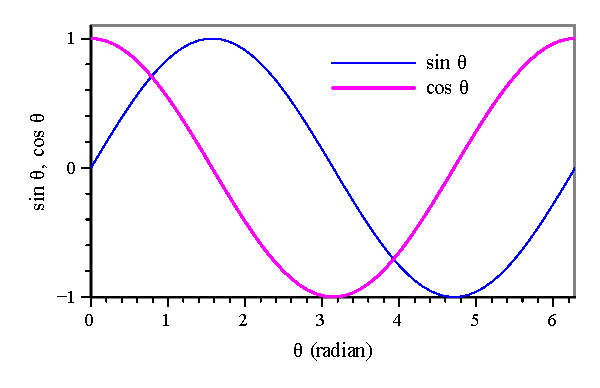
\includegraphics[width=0.75\linewidth]{fig3_1}
\caption[ % Short title which ia appear in figures list
توابع سینوس و کسینوس در یک دورهٔ تناوب]{ % عنوان بلند که زیر شکل می‌آید
توابع سینوس 
(\textcolor{blue}{منحنی نازک}) 
و کسینوس 
(\textbf{\textcolor{magenta}{منحتی ضخیم}}) 
در یک دورهٔ تناوب برحسب زاویه.}
\label{fig3:1}
\end{figure}

شکل~%
\ref{fig3:1} 
نمونه‌ای ساده است که توابع سینوس و کسینوس را در یک دورهٔ تناوب نشان می‌دهد. راهنمای شکل حتی در چاپ سیاه سفید قابل استفاده است. محورها به گونه‌ای مدرج شده اند که پیدا کردن مقادیر ساده است و در عین حال شلوغ نیستند.

وقتی جزییات یک شکل زیاد نباشد، می‌توان عرض آن را کاهش داد و عنوان را کنار آن آورد. شکل~%
\ref{fig3:2} 
همان شکل~%
\ref{fig3:1} 
است که عرض آن کاهش یافته است. اما اندازه قلم به همان نسبت بزرگ شده تا اعداد و نوشته‌ها واضح باشند.

\begin{figure}[!tbhp] % Fig. 3:2
\thisfloatsetup{capbesideposition={center,outside},capbesidewidth=6cm,facing=yes}
\fcapside[\FBwidth]{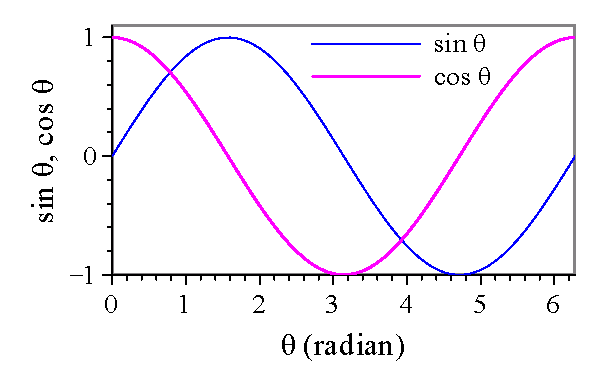
\includegraphics[width=\linewidth]{fig3_2}}{
\caption[ % Short title which ia appear in figures list
توابع سینوس و کسینوس در یک دورهٔ تناوب]{ % عنوان بلند که زیر شکل می‌آید
توابع سینوس 
(\textcolor{blue}{منحنی نازک}) 
و کسینوس 
(\textbf{\textcolor{magenta}{منحتی ضخیم}}) 
در یک دورهٔ تناوب برحسب زاویه. عرض شکل کاهش یافته تا عنوان کنار شکل جا شود.}
\label{fig3:2}}
\end{figure}

همیشه در انتخاب نسبت ابعاد شکل آزاد نیستیم. مثلاً در تصاویر میکروسکپی که با سی‌سی‌دی ثبت می‌شوند، این نسبت براساس سخت‌افزار مشخص می‌شود و نباید آن را تغییر داد. شکل~%
\ref{fig3:3} 
نمونه‌ای از این تصاویر است. شما فقط می‌توانید اندازه شکل را به گونه‌ای تنظیم کنید که همه چیز واضح باشد. فراموش نکنید که این تصاویر باید با میله مقیاسی مدرج شوند که مقیاس واقعی آنها را مشخص کند.

\begin{figure}[!tbhp] % Fig. 3:3
\centering
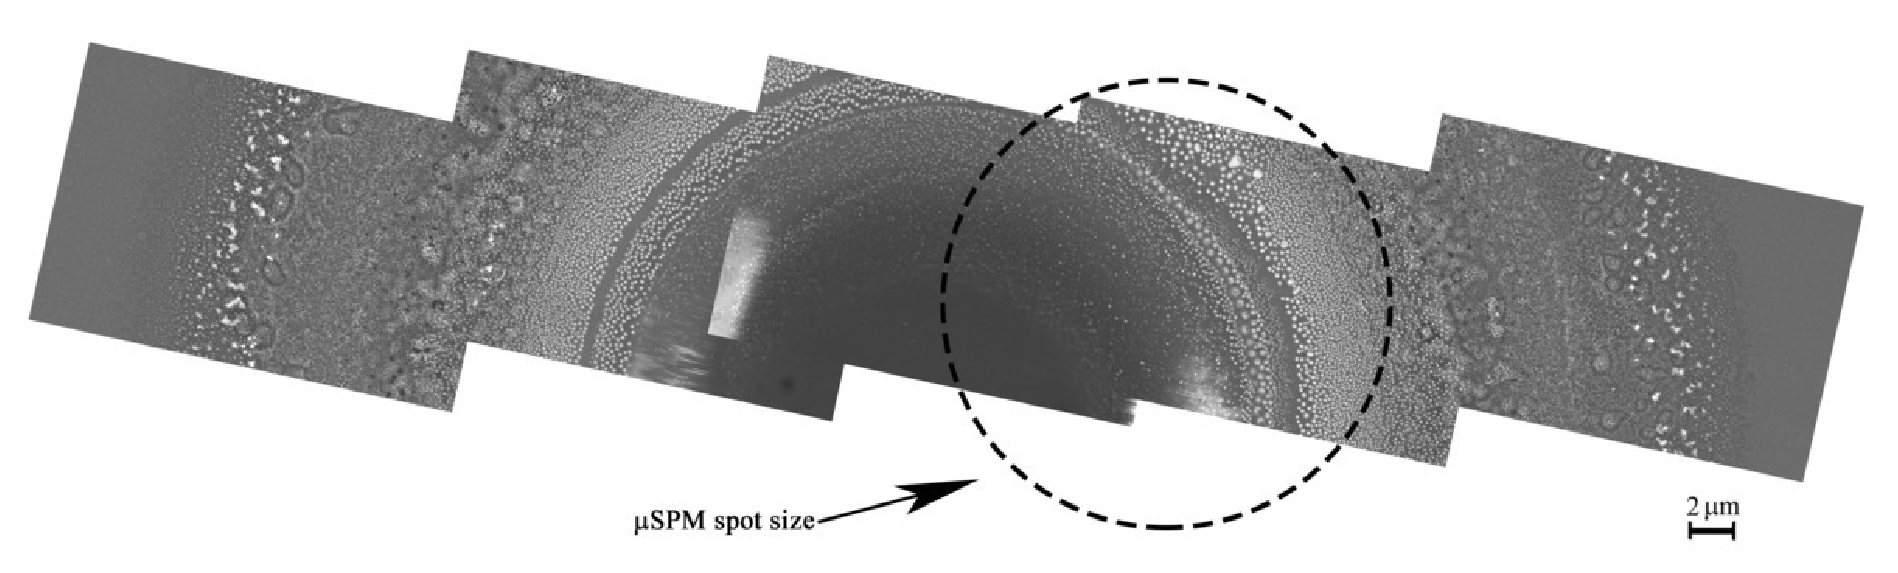
\includegraphics[width=0.9\linewidth]{fig3_3}
\caption[ % Short title which ia appear in figures list
تصویر میکروسکوپی الکترونی از نانوذرات نقره در شیشه تبادل‌یون شده]{ % عنوان بلند که زیر شکل می‌آید
تصویر میکروسکوپی الکترونی از نانوذرات نقره در سطح و ماتریس شیشه تبادل‌یون شدهٔ سودا\dash لایم، برگرفته از مرجع 
\citenum{Ahangary2010}. 
این تصویر عریض از کنارهم قرار دادن و منطبق کردن تعدادی تصویر ساخته شده است.}
\label{fig3:3}
\end{figure}

گاهی نیاز است بیش از یک نمودار یا تصویر در یک شکل گنجانده شوند. شکل~%
\ref{fig3:4} 
چنین نمونه‌ای را نشان می‌دهد. اگر بتوان نسبت ابعاد را به دلخواه انتخاب کرد، بهتر است برای دو شکل قدی کنار هم، نسبت ارتفاع به طول
$1.4$ 
باشد. این نسبت برای سه شکل قدی کنار هم، 
$1.7$ 
است. به این ترتیب نسبت ابعاد هر شکل و کل مجموعه تا حد ممکن مقداری نزدیک به نسبت طلایی خواهند داشت.

\begin{figure}[!tbhp] % Fig 3:4
	\begin{subfigure}[b]{0.35\linewidth}
	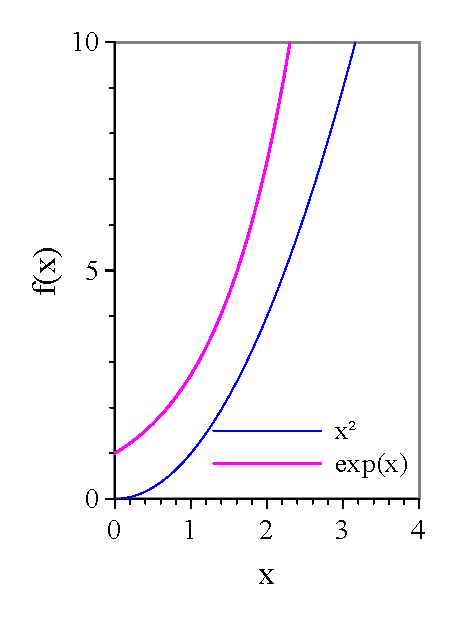
\includegraphics[width=\linewidth]{fig3_4a.eps}
	\caption{}
	\end{subfigure}\qquad
	\begin{subfigure}[b]{0.35\linewidth}
	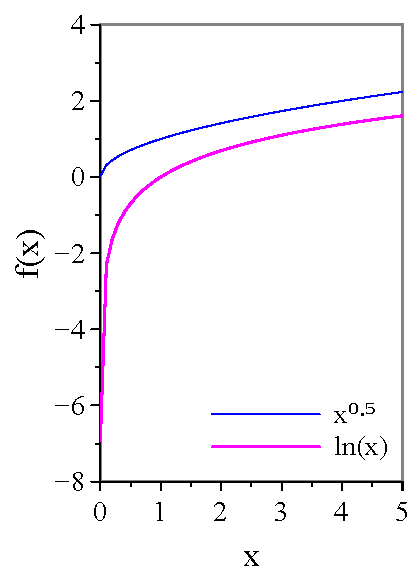
\includegraphics[width=\linewidth]{fig3_4b.eps}
	\caption{}
	\end{subfigure}
\caption[ % Short title which ia appear in figures list
مقایسه رشد سریع تابع نمایی با مربع و رشد کند لگاریتم با جذر]{ % عنوان بلند که زیر شکل می‌آید
(آ) مقایسه رشد سریع تابع نمایی 
(\textbf{\textcolor{magenta}{منحتی ضخیم}}) 
نسبت به توان دوم (مربع) 
(\textcolor{blue}{منحنی نازک}).
(ب) مقایسه رشد کند تابع لگاریتم 
(\textbf{\textcolor{magenta}{منحتی ضخیم}}) 
در مقایسه با جذر 
(\textcolor{blue}{منحنی نازک}).}
\label{fig3:4}
\end{figure}

همیشه نسبت ابعاد در اختیار ما نیست. حتی ممکن است بخواهیم دو شکل با نسبت ابعاد نامساوی را کنار هم بیاوریم. در این موارد بهتر است ارتفاع شکل‌ها را تنظیم کنیم و اجازه دهیم با طول نامساوی کنار هم قرار گیرند، شکل~%
\ref{fig3:5}.


\begin{figure}[!tbhp] % Fig 3:5
	\begin{subfigure}[b]{0.25\linewidth}
	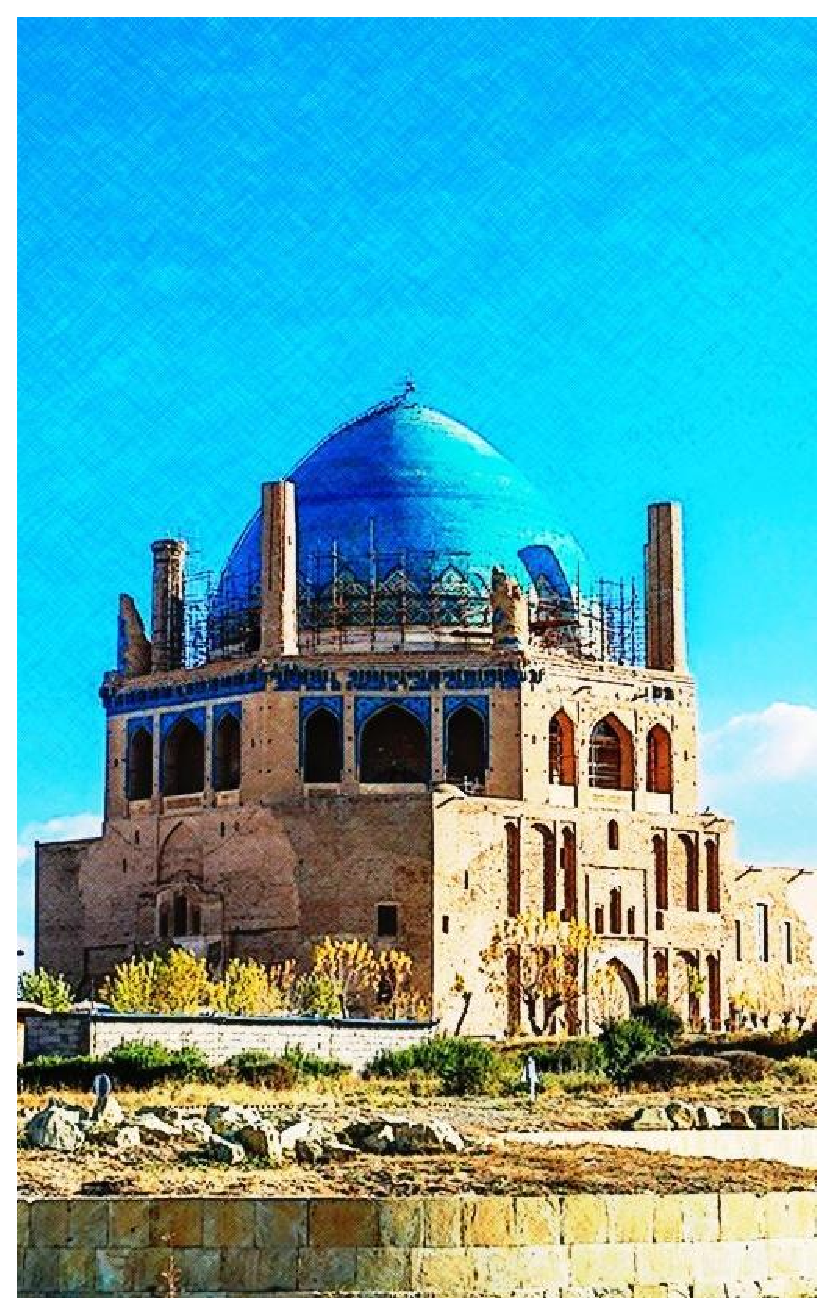
\includegraphics[height=6cm]{fig3_5a.eps}
	\caption{}
	\end{subfigure}\qquad
	\begin{subfigure}[b]{0.55\linewidth}
	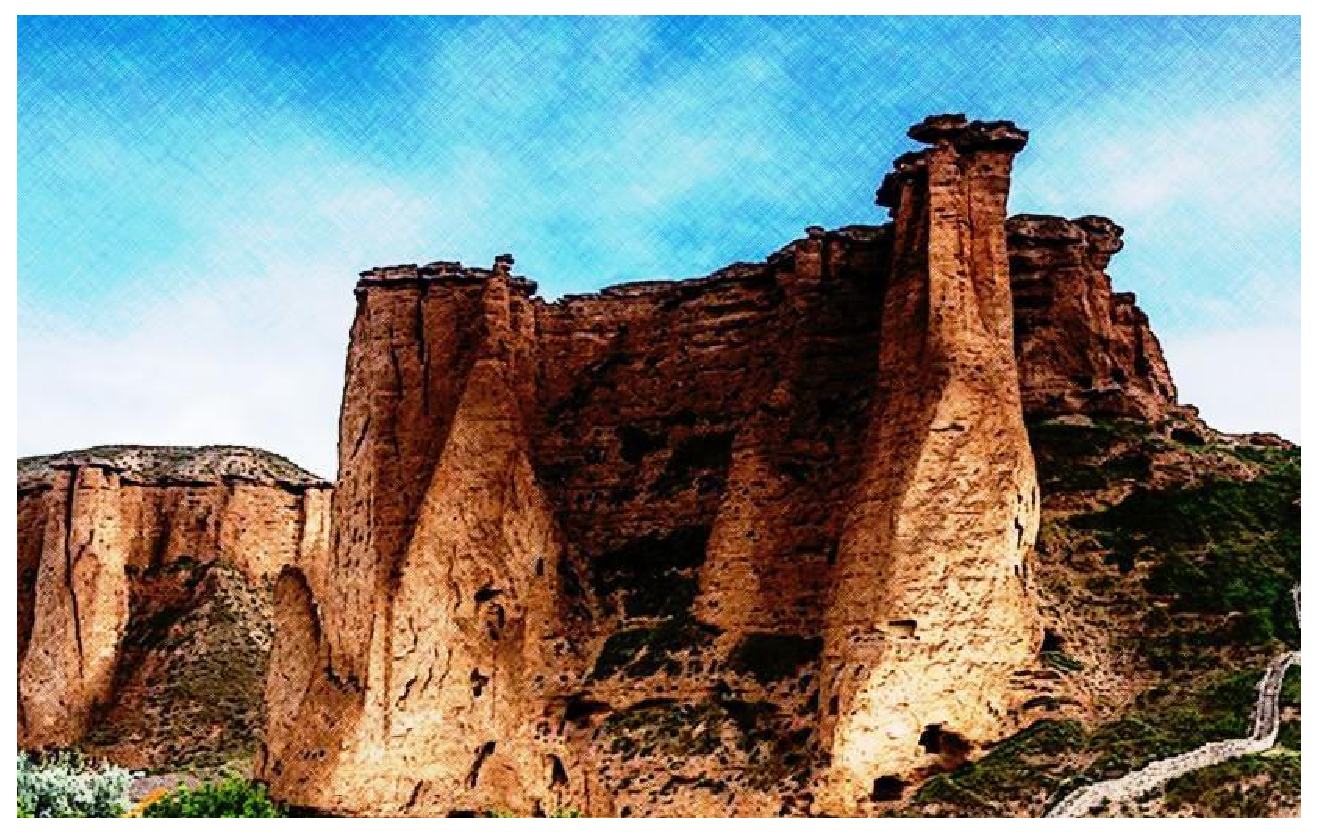
\includegraphics[height=6cm]{fig3_5b.eps}
	\caption{}
	\end{subfigure}
\caption[ % Short title which ia appear in figures list
تصاویری از جاذبه‌های گردشگری زنجان]{ % عنوان بلند که زیر شکل می‌آید
تصاویری از جاذبه‌های گردشگری استان زنجان، (آ) گنبد آجری سلطانیه، (ب) دودکش جن در نزدیکی شهرستان ماهنشان.}
\label{fig3:5}
\end{figure}

گاهی با شرایطی روبرو هستیم که سه نمودار مربوط به هم داریم که می‌خواهیم آنها را در قالب یک شکل ترکیب کنیم. جزئیات شکل‌ها آنقدر زیاد است که نمی‌توان آنها را کوچک کرد و هر سه را در یک سطر کنار هم چید. ترجیح می‌دهیم آنها را در یک ساختار 
$2\times2$ 
جای دهیم. اما سه شکل بیشتر نداریم و جای خالی چهارم زیبا نخواهد بود. در این موارد می‌توان جای خالی را با عنوان شکل‌ها پر کرد. شکل~%
\ref{fig3:6} 
نمونه‌ای از این شرایط را نشان می‌دهد.

\begin{figure}[!tbhp] % Fig 3:6
  \begin{subfloatrow}[2]
    \floatrowsep\quad
    \ffigbox{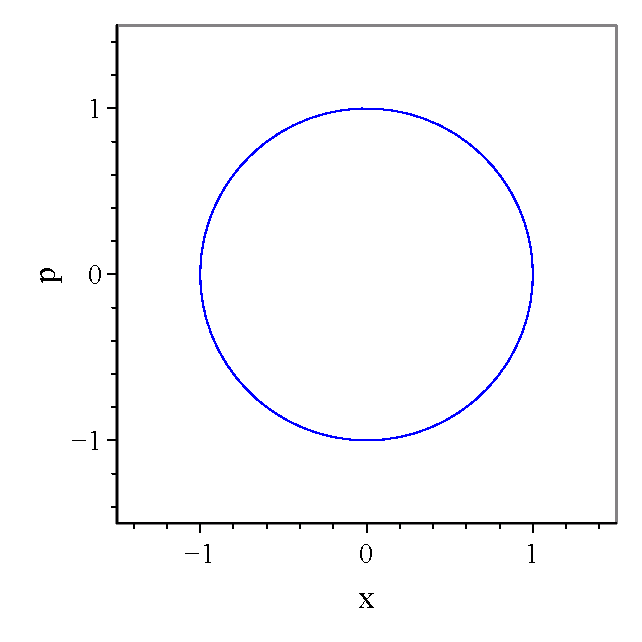
\includegraphics[width=0.45\textwidth]{fig3_6a.eps}}{\subcaption{}}
    \ffigbox{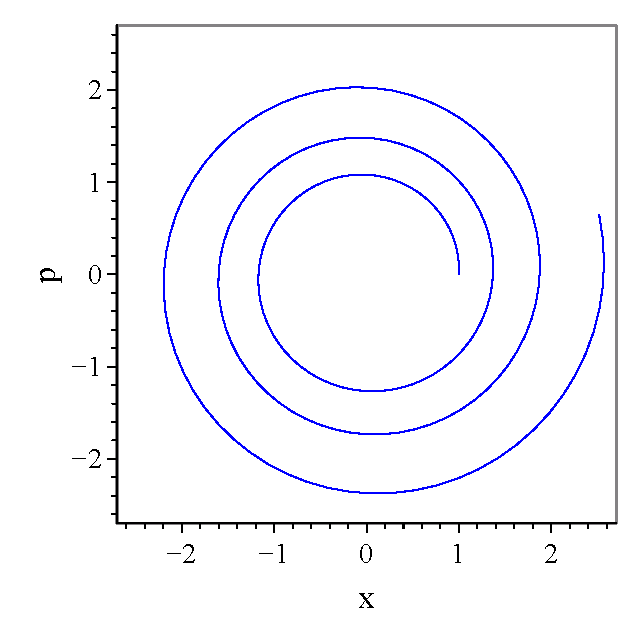
\includegraphics[width=0.45\textwidth]{fig3_6b.eps}}{\subcaption{}}
  \end{subfloatrow}
  \begin{subfloatrow*}[2]
    \floatrowsep\quad
    \ffigbox{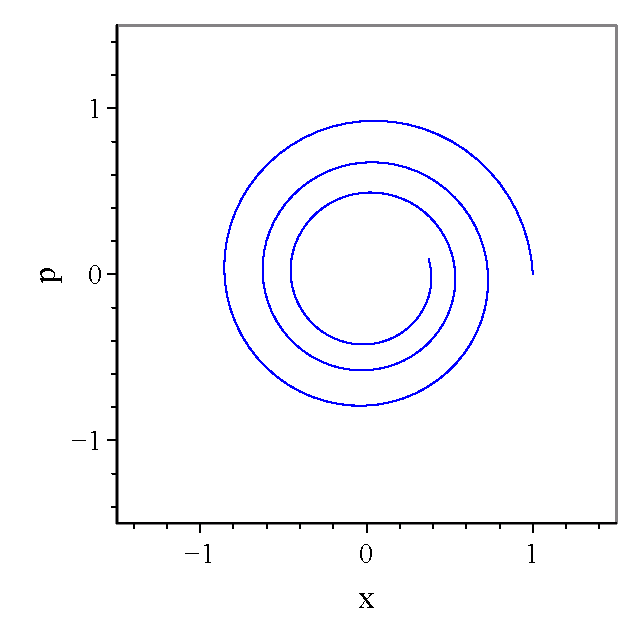
\includegraphics[width=0.45\textwidth]{fig3_6c.eps}}{\subcaption{}}
    \captionsetup{position=top}
    \ffigbox[][][t]{}{
    \RawCaption{\caption[ % Short title which ia appear in figures list
منحنی فاز نوسانگر در سه حالت ایده‌آل، واداشته بدون اتلاف، و اتلافی]{ % عنوان بلند که زیر شکل می‌آید
(آ) منحنی فاز نوسانگر در شرایط ایده‌آل و بدون اتلاف که انرژی ثابت است و نمودار فاز در واحدهای کاهیده دایره‌ای با شعاع واحد است، (ب) منحنی فاز نوسانگر واداشته با اتلاف ناچیز که انرژی آن با زمان افزایش می‌یابد به‌صورت مسیری مارپیچ است که شعاع آن رو به افزایش است. (ج) منحنی فاز نوسانگر اتلافی که انرژی با زمان کاهش می‌یابد و شعاع مسیر مارپیچ به مرور کاهش می‌یابد.}
    \label{fig3:6}}}
  \end{subfloatrow*}
\end{figure}

پیش می‌آید که تعداد زیادی نمودار مرتبط به هم داریم و مایلیم آن‌ها را کنار هم نشان دهیم، مثلاً شکل~\ref{fig3:7}. این نمودارها ممکن است جنبه‌های مختلف یک حل یا شبیه‌سازی را نشان دهند که مایل باشیم همزمان دیده شوند. اما رسم آنها کنار هم سبب شود خیلی کوچک نمایش داده شوند و جزئیات قابل مشاهده نباشد. یک راه‌حل ابتکاری این است که نمودارها را طوری کنار هم بچینیم که محورهای افقی و عمودی مشابه را بتوان به‌صورت مشترک رسم کرد. به این ترتیب با حذف محورهای تکراری بخشی از فضا آزاد می‌شود و می‌توانید نمودارها را اندکی بزرگ‌تر و واضح‌تر رسم کنید. در این مورد بهتر است نمودارها را همسان و همانند هم رسم کنید و کار برش بخش‌های اضافی محورها را در خود 
\latex 
انجام دهید تا هماهنگ کردن تصاویر ساده‌تر شود.

\begin{figure}[!tbhp] % Fig 3:7 
  \begin{subfloatrow}[3]
    \ffigbox{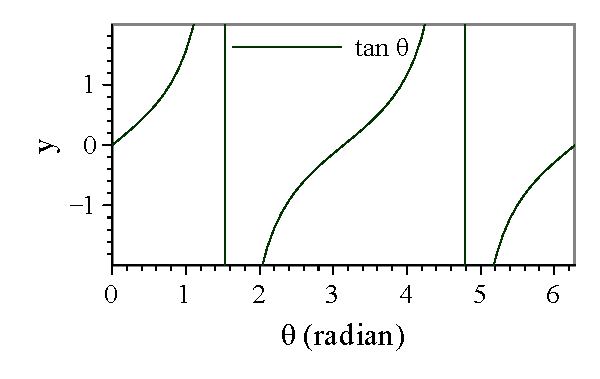
\includegraphics[width=1.26\linewidth,trim= 0 1.5cm 0 0,clip]{fig3_7a.eps}}{}~~~~~~~~~
    \ffigbox{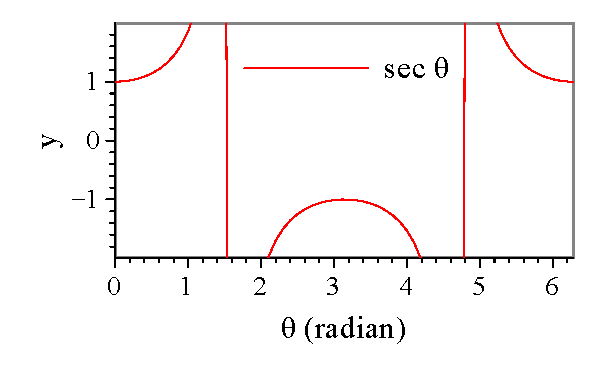
\includegraphics[width=1.06\linewidth,trim= 1.5cm 1.5cm 0 0,clip]{fig3_7b.eps}}{}
    \ffigbox{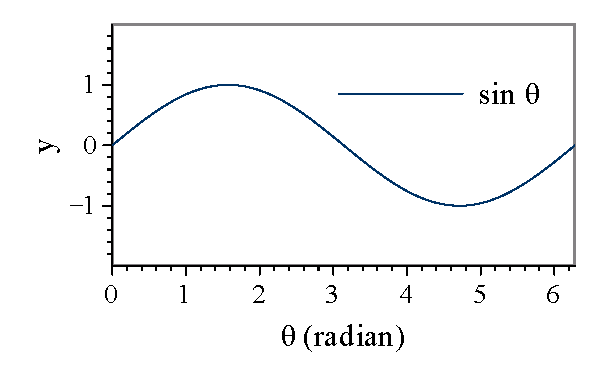
\includegraphics[width=1.06\linewidth,trim= 1.5cm 1.5cm 0 0,clip]{fig3_7c.eps}}{}
  \end{subfloatrow}
  \begin{subfloatrow}[3]
    \ffigbox{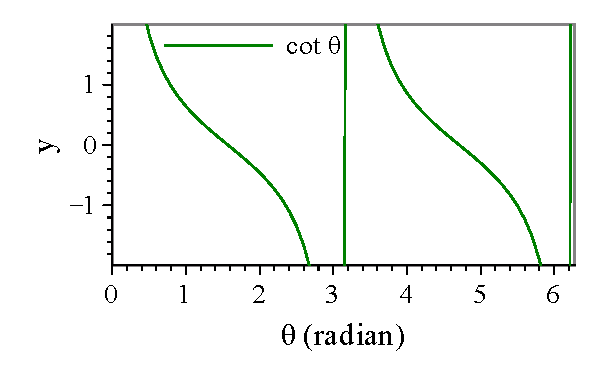
\includegraphics[width=1.26\linewidth,trim= 0 0 0 0,clip]{fig3_7d.eps}}{}~~~~~~~~~
    \ffigbox{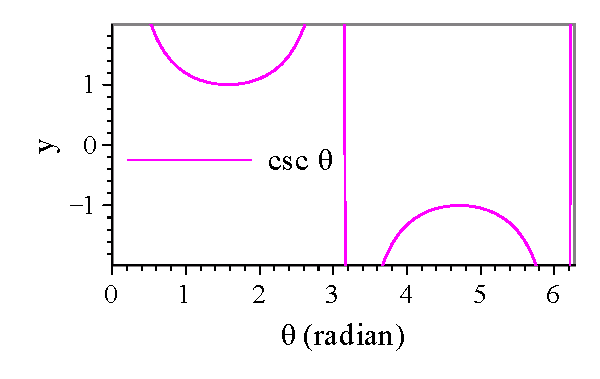
\includegraphics[width=1.06\linewidth,trim= 1.5cm 0 0 0,clip]{fig3_7e.eps}}{}
    \ffigbox{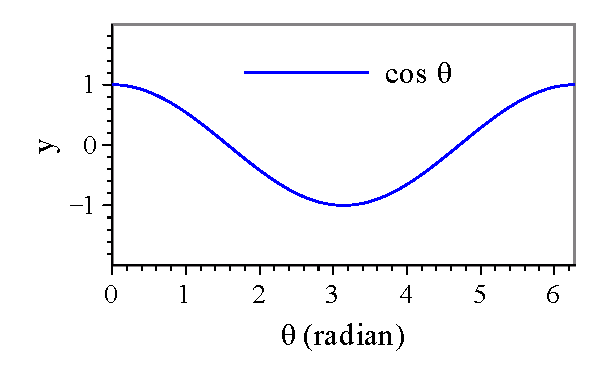
\includegraphics[width=1.06\linewidth,trim= 1.5cm 0 0 0,clip]{fig3_7f.eps}}{}
  \end{subfloatrow}
  \RawCaption{\caption[ % Short title which ia appear in figures list
منحنی تغییرات توابع مثلثاتی در یک دوره تناوب]{ % عنوان بلند که زیر شکل می‌آید
منحنی تغییرات تابع (بالا راست) سینوس، (بالا وسط) سکانت، (بالا چپ) تانژانت، (پایین راست) کسینوس، (پایین وسط) کسکانت، و (پایین چپ) کتانژانت در یک دورهٔ تناوب.}
  \label{fig3:7}}
\end{figure}

وضعیت‌هایی پیش می‌آید که می‌خواهید یک نقشه یا طرح مهم با جزئیات فراوان را نشان دهید و نمایش آن حتی به صورت تنها (نظیر شکل~%
\ref{fig3:1}) 
به اندازه کافی بزرگ و واضح نیست. این شرایط وقتی پیش می‌آید که نسبت طول به ارتفاع شکل بزرگتر است. در این موارد می‌توانید شکل را $90^\circ$ بچرخانید و آن را تنها در یک صفحه کامل بیاورید، شکل~%
\ref{fig3:8}. 
به این ترتیب طول شکل در امتداد ارتفاع صفحه کاغذ که بزرگ‌تر است قرار می‌گیرد و شکل بزرگ‌تر و واضح‌تر دیده می‌شود.

\begin{sidewaysfigure} % Fig. 3:8
\centering
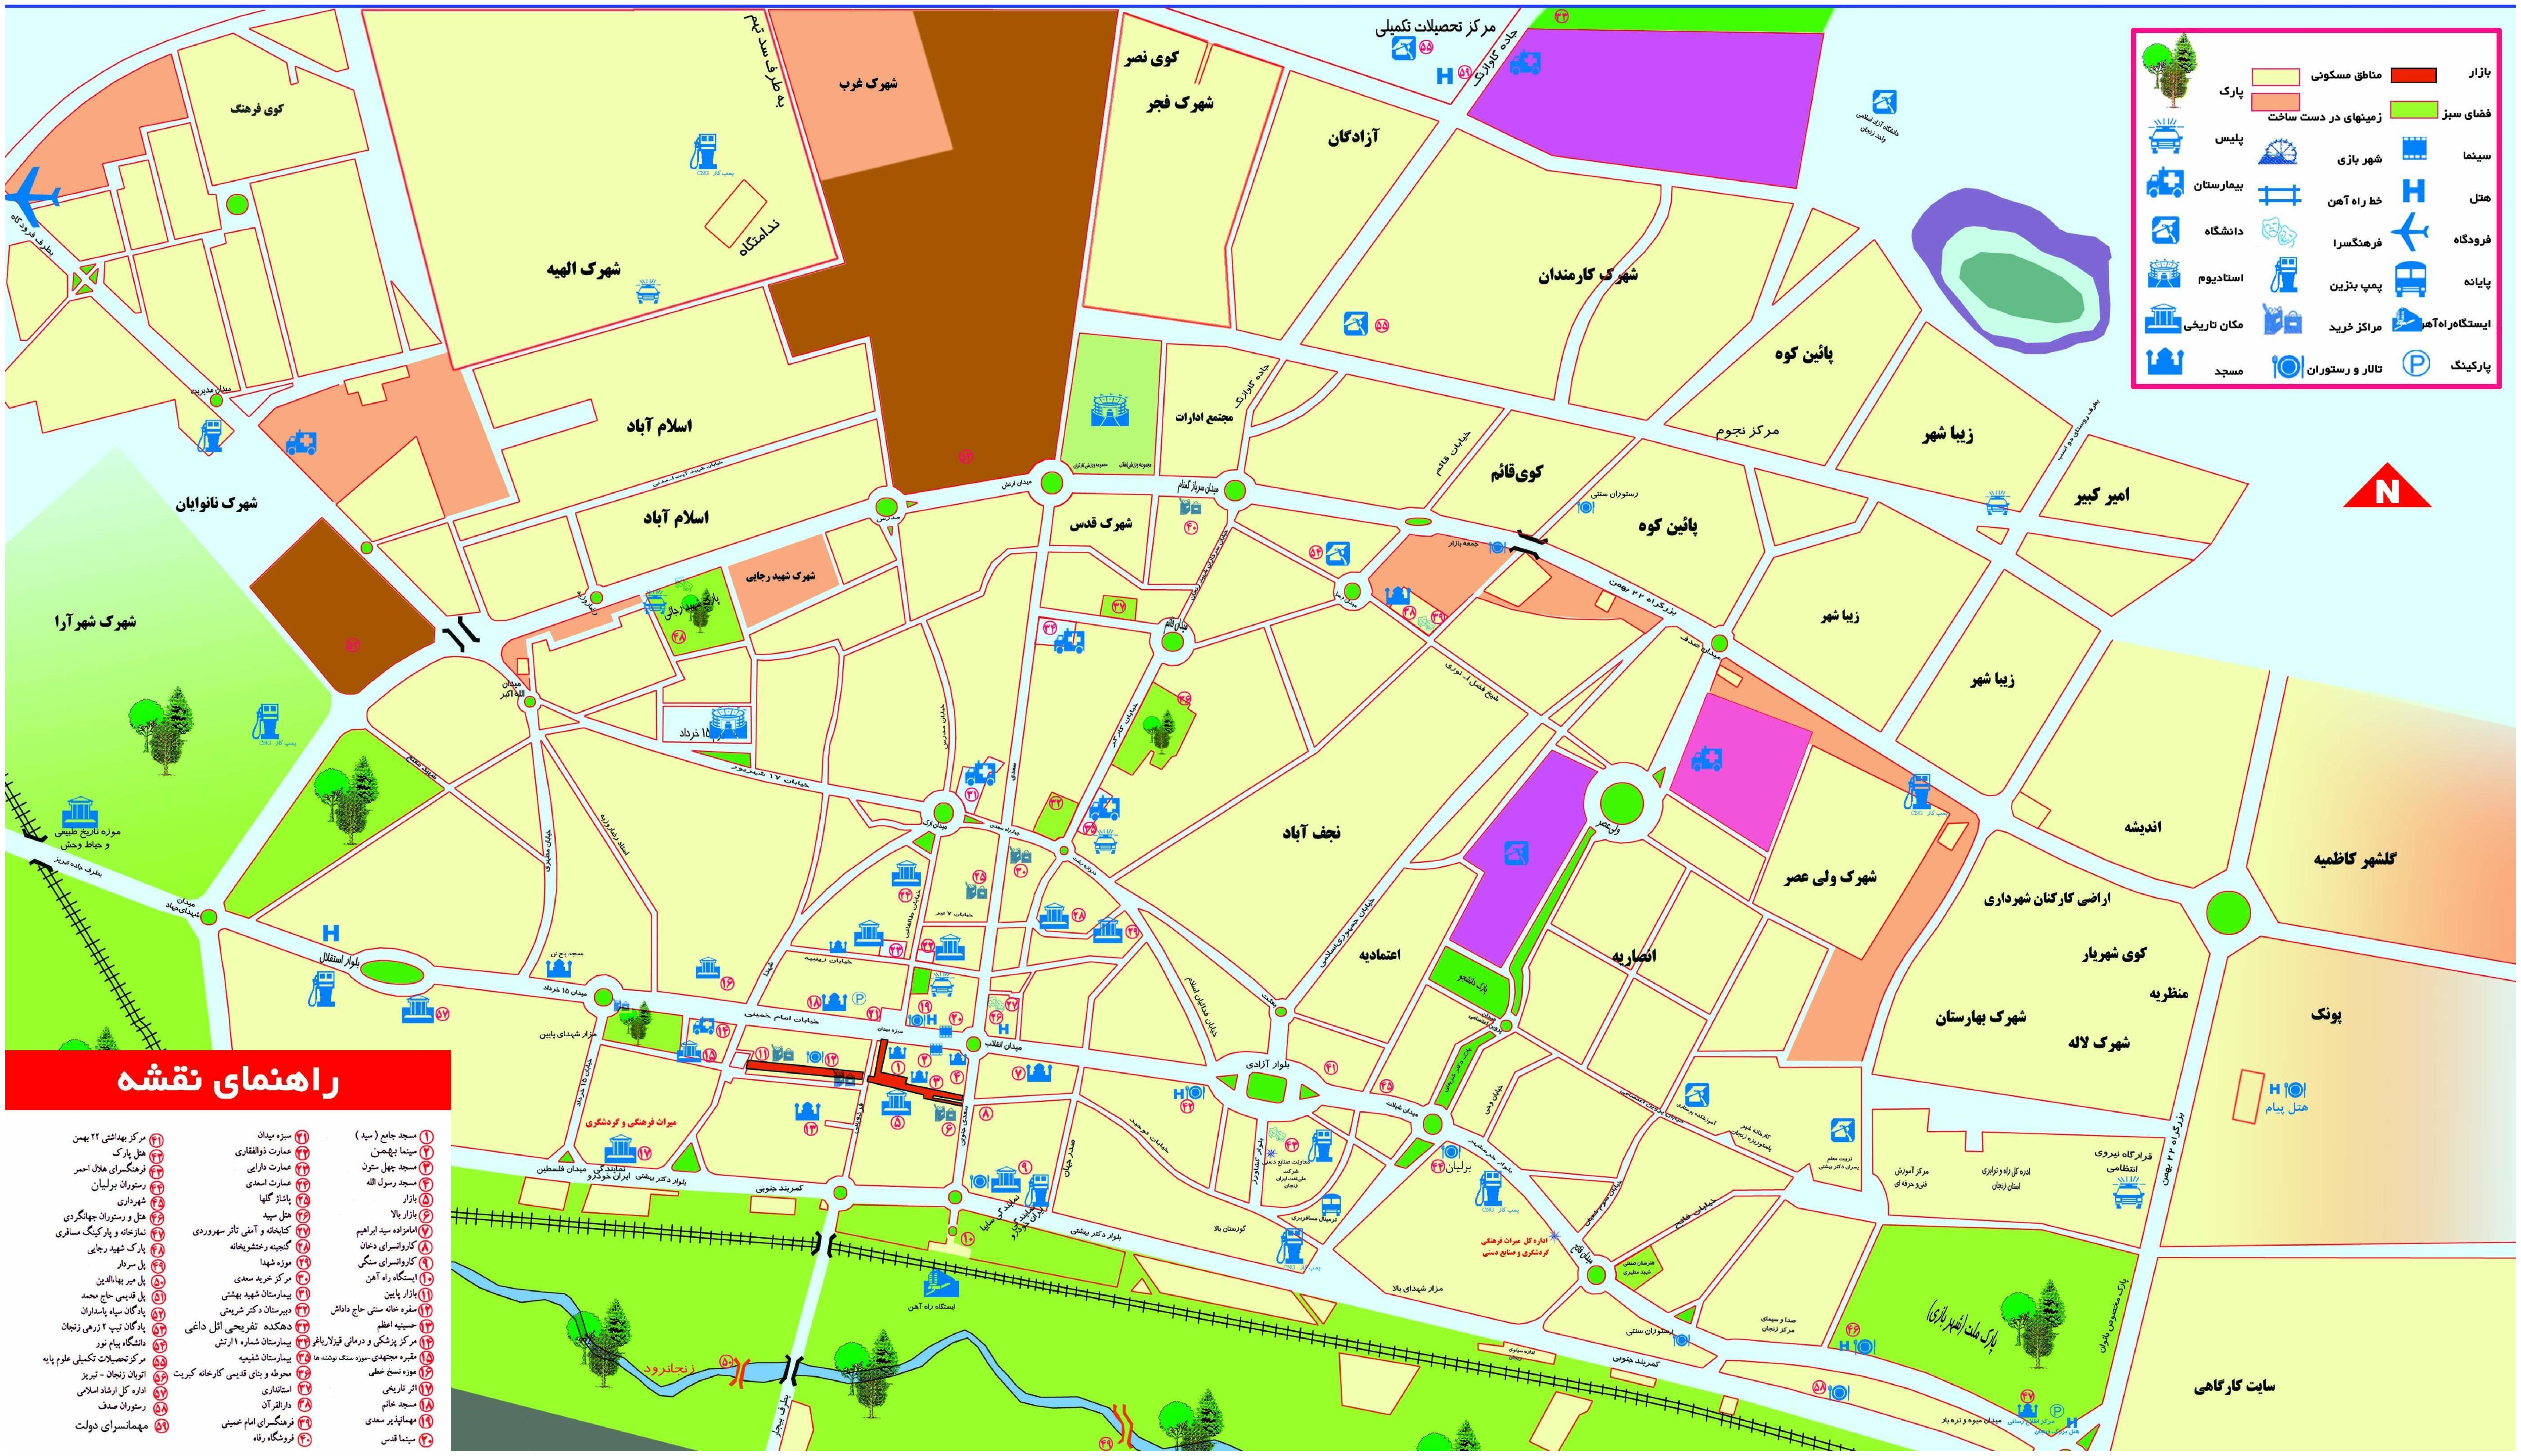
\includegraphics[width=\linewidth]{fig3_8}
\caption[ % Short title which ia appear in figures list
نقشه راهنمای شهر زنجان]{ % عنوان بلند که زیر شکل می‌آید
نقشه راهنمای شهر زنجان، اداره میراث فرهنگی، صنایع دستی و گردشگری استان زنجان.}
\label{fig3:8}
\end{sidewaysfigure}

در این الگو برای کنار هم چیدن شکل‌ها و جدول‌ها، همزمان از بسته‌های 
\lr{subfigure} و \lr{floatrow} \latex 
استفاده شده است. می‌توانید ترکیبات پیچیده‌تر را با مطالعهٔ راهنمای این دو بسته‌ ایجاد کنید. روش ساده‌تر این است که از هوش مصنوعی کمک بگیرید و به دلخواه خودتان ترکیبات پیچیده‌تری را ایجاد کنید. این الگو تسلیم خلاقیت و ابتکار شما است و قصدی برای محدود کردن شما ندارد.


\section{اضافه کردن جدول‌ها}
ممکن است 
\thesis 
شما اصلاً شامل شکل و جدول نباشد. در این صورت به فهرست اشکال و جداول نیز نیاز ندارد. این الگو به‌صورت خودکار با اضافه شدن اولین شکل و جدول، به ترتیب فهرست اشکال و جدوال را به 
\thesis 
اضافه می‌کند. 

جدول~%
\ref{tab3:1} 
نمونه‌ای از یک جدول است که با حذف خطوط افقی و عمودی به زیبایی آن افزوده شده است.

\begin{table}[!htbp] % Table 3:1
\caption{\small
برخی پیشوندها در دستگاه اندازه‌گیری 
\lr{SI}.}\label{tab3:1}
\begin{center}\small\begin{tabular}{rcl} 
\hline\noalign{\smallskip}
\textbf{
نام پیشوند} & \textbf{حرف اختصاری} & \textbf{مقدار}\\[4pt] 
\hline\noalign{\smallskip}
دسی
& $\mathrm{d}$ & $10^{-1}$\\
سانتی
& $\mathrm{c}$ & $10^{-2}$\\
میلی
& $\mathrm{m}$ & $10^{-3}$\\
میکرو
& $\mu$        & $10^{-6}$\\[4pt]
\hhline{===}
\end{tabular}\end{center}
\end{table}

برخی مواقع لازم است که دو یا چند خانه جدول باهم ادغام شوند. مثلاً در جدول~%
\ref{tab3:2}، 
دو خانه اول در سطر اول سرایند جدول ادغام شده‌اند. در دو ستون بعدی نیز خانه‌ها در دو سطر متوالی با هم ادغام شده اند تا سرآیند جدول زیباتر شود.

\begin{table}[!htbp] % Table 3:2
\small\caption{
برخی مقادیر و ثابت‌های فیزیکی.}
\label{tab3:2}
\begin{tabular}{rcll} 
\hline\noalign{\smallskip}
\multicolumn{2}{c}{\textbf{
ثابت‌های فیزیکی}} & 
\multirow{2}{*}{\textbf{مقدار}} & 
\multirow{2}{*}{\textbf{نماد}}\\[4pt]
\hhline{--} \noalign{\smallskip}
نام & توضیحات \\[4pt]
\hline \noalign{\smallskip}
سرعت نور & در خلا &
$3 \times 10^8\unit{m/s}$ & $c$\\
\multicolumn{2}{r}{
ثابت پلانک} & 
$6.626 \times 10^{-34}\unit{Js}$ & $h$\\
جرم الکترون & در حالت سکون & 
$9.109 \times 10^{-31}\unit{kg}$ & $m_\mathrm{e}$\\[4pt]
\hline
\end{tabular}
\end{table}

همانند شکل‌ها، ممکن است با جدول‌هایی روبرو شوید که تعداد زیادی ستون داشته باشند. به‌عبارتی تعداد ستون‌ها و عرض آنها در مجموع بیش از عرض صفحه باشد. بهتر است برای جادادن چنین جداولی در صفحه، جدول را $90^\circ$ بچرخانید و یک صفحه کامل به آن اختصاص دهید. کافیست به‌جای محیط 
\lr{table} 
از محیط 
\lr{sidewaystable} 
استفاده کنید،~\ref{tab3:3}.

\begin{sidewaystable} % Table 3:3
\small\caption[ % Short title which ia appear in figures list
حالت‌های متنوع کلاس\dash سند \lr{`iasbs-thesis'}.]{ % عنوان بلند که زیر شکل می‌آید
حالت‌های متنوع کلاس\dash سند \lr{`iasbs-thesis'} و چیدمان صفحات برمبنای انتخاب آنها.}
\label{tab3:3}
\newcommand{\vr}[1]{\rotatebox{90}{\small #1}}
\begin{tabular}{rc ccccc c ccc cccc c} 
\hline\noalign{\smallskip}
\multirow{2}{*}{\parbox{6em}{\vspace{8em}\centering\textbf{
نوع سند}}} & 
\multirow{2}{*}{\parbox{10em}{\vspace{8em}\centering\textbf{
گزینه‌های انتخاب شده}}} & 
\multicolumn{14}{c}{\textbf{شمارهٔ صفحه}$\,\!^*$}\\[4pt] 
\hhline{~~----- - --- ---- -}\noalign{\smallskip}
&& \vr{جلد} & \vr{عنوان فارسی} & \vr{عنوان انگلیسی} & \vr{شناسنامه} & \vr{کپی‌رات} & 
   \vr{بسم الله الرحمن الرحیم} & 
   \vr{اعلامیه} & \vr{تأییدیه فارسی} & \vr{تأییدیه انگلیسی} & 
   \vr{تقدیم به} & \vr{قدردانی} & \vr{چکیده فارسی} & \vr{چکیده انگلیسی} & 
   \vr{فهرست‌ها}\\
\hline \noalign{\smallskip}   
پیش‌نویس رسالهٔ دکتری & \lr{phd + review} & 
1 & 3 & 4 & 5 & 6 &   8 &   9 & 10 & 11 &   12 & 13 & 14 & 15 & 16\\[4pt]
رسالهٔ دکتری & \lr{phd} & 
\lr{ix} & 1 & \lr{vii} & 2 & \lr{iii} &   3 &   5 & 7 & \lr{v} &   9 & 11 & 13 & \lr{i} & 15\\[4pt]
پیشنهاد رسالهٔ دکتری & \lr{phd + proposal} &
- & 1 & \lr{} & 2 & \lr{i} &   3 &   - & - & - &   - & - & 5 & - & 7\\[4pt]
پیش‌نویس پایان‌نامهٔ کارشناسی ارشد & \lr{master + review} &
1 & 3 & 4 & 5 & - &   6 &   - & 7 & 8 &   10 & 11 & 12 & 13 & 14\\[4pt]
پایان‌نامهٔ کارشناسی ارشد & \lr{master} & 
\lr{xii} & 1 & \lr{v} & 2 & - &   3 &   - & 5 & \lr{iii} &   7 & 9 & 11 & \lr{i} & 13\\[4pt]
گزارش پروژه کارشناسی & \lr{-} &
- & 1 & \lr{i} & - & - &   - &   - & - & - &   - & - & 3 & \lr{} & 5\\[4pt]
\hline \noalign{\smallskip}
\multicolumn{14}{r}{$\,\!^*$
شمارهٔ یونانی مشخص می‌کند آن صفحه در انتهای \thesis می‌آید.}
\end{tabular}
\end{sidewaystable}


\section{تسهیل نگارش اصطلاحات علمی}
در یک متن علمی، واژگان و اصطلاحات زیادی وجود دارد که باید به نحو مناسب از معادل فارسی یا  مخفف آنها استفاده کنید. گاهاً معادل فارسی این اصطلاحات خیلی طولانی است و برای آنها همانند انگلیسی مخفف نداریم یا شما مطمئن نیستید که مخففی که قصد استفاده از آن را دارید با اقبال داوران روبرو شود. در اینجا چند مثال از دستورات 
\latex 
می‌آوریم که می‌توانید ابتدای فایل اصلی 
\thesis (\lr{``main.tex"}) 
قبل از محیط 
$\backslash\texttt{begin\{documnet\}}$
بیاورید و برای تسهیل نگارش چنین اصلاحاتی از آنها استفاده کنید. 

برای مثال در انگلیسی معمولاً 'روش افت‌وخیز روندزدایی شده%
\LTRfootnote{Detrended Fluctuation Analysis (DFA)}` 
به اختصار 
\lr{DFA} 
نوشته می‌شود. تکرار کردن این اصطلاح طولانی و درست نوشتن فاصله‌ها و نیم‌فاصله‌های آن دشوار و خسته کننده است. اگر دستور کوتاهی در 
\latex 
این اصطلاح طولانی را برای ما تولید کند خیلی راحت‌تر است. کافی است کد زیر در ابتدای کد اصلی اضافه شود تا دستور 
'$\backslash\texttt{dfa}$` 
این کار را برایمان انجام دهد،
\begin{latin}
\noindent$\backslash\texttt{newcommand}\{\backslash\texttt{dfa}\}\{
\mbox{\small\rl{
افت‌وخیز روندزدایی شده}}%
\!\backslash\texttt{xspace}\}$
\end{latin}

مثال دیگری که می‌توان زد اصطلاح 'دینامیک مولکولی%
\LTRfootnote{Molecular Dynamics (MD)}` 
است. در انگلیسی این اصطلاح را به اختصار 
\lr{MD} 
می‌نویسند. ممکن است در زمان نگارش 
\thesis 
واژهٔ 'دینامول` به عنوان مخفف فارسی 'دینامیک مولکولی` به ذهنمان برسد، اما از نظر مساعد داوران مطمئن نباشیم. راه‌حل تعریف دستور 
'$\backslash\texttt{md}$`
در ابتدای فایل اصلی است،
\begin{latin}
\noindent$\backslash\texttt{newcommand}\{\backslash\texttt{md}\}\{
\mbox{\small\rl{
دینامول}}%
\!\backslash\texttt{xspace}\}$
\end{latin}
\noindent
به این ترتیب هم نگارش آن به اندازه نسخهٔ انگلیسی ساده است و هم فرصت خواهیم داشت در آینده در نحوه نگارش آن تجدید نظر کنیم.

مورد آخر وقتی است که می‌خواهیم یک واژه را به صورت خاصی بنویسیم. مثلاً برای خوانش درست اعراب‌گذاری کنیم، یا جلوه هنری یا فانتزی به آن بدهیم و این کار پیچیدگی‌هایی دارد که نمی‌خواهیم هر بار آن را تکرار کنیم. نمونه‌های آن لوگوهای
\latex، \xelatex، 
و 
\xepersian 
به فارسی است که از نمونه انگلیسی آنها برداشت شده است (
\LaTeX، \XeLaTeX، و \XePersian). 
این مثال اگرچه جایی در متن 
\thesis{ٔ} 
شما ندارد، اما قابلیت‌هایی را در نگارش متن نمایش می‌دهد که ممکن است به کارتان بیاید. برای مشاهده تعریف دستوراتی که این لوگوهای فارسی را تولید می‌کند، به فایل 
'$\texttt{main.tex}$` 
مراجعه کنید.


\section{یاداشت‌گذاری}
زیاد پیش می‌آید که توصیه‌هایی از استاد راهنما یا مشاور دریافت کنید یا نکاتی به ذهنتان برسد، اما همان موقع نتوانید آنها را رفع کنید و مایل باشید برای یادآوری کارهایی که باید انجام دهید، در متن یادداشت بگذارید. این کار با بسته \lr{easyReview} قابل انجام است. مزیت این بسته آن است که در نوار ابزار نرم‌افزار استودیوی‌تک%
\LTRfootnote{TeXstudio} 
از پیش گزینه‌هایی برای فراخوانی دستورات این بسته وجود دارد. با این بسته می‌توانید کارهای زیر را انجام دهید:

\begin{itemize}
\item 
پیام 
\alert{%
هشداری} را در متن نمایش دهید تا فراموش نشود.
\item 
\add{%
متن جدید اضافه شده به متن اصلی} را مشخص کنید.
\item 
متن حذف شده از متن اصلی
\remove{%
متن اضافی} را مشخص کنید. 
\item
مشخص کنید که کجا 
\replace{%
متنی جایگزین}{متنی دیگر} شده است.
\item
قسمتی از
\highlight{%
متن را هایلایت} کنید تا بعداً به آن توجه کنید.
\item 
توضیحاتی را به متن اصلی اضافه کنید: 
\comment{%
مثلاً این جمله نیاز به کامنت و توضیح دارد که در جعبه زیر متن ظاهر می‌شود.}{نکته: هر زمان مایل باشید می‌توانید توضیحات و تاریخچه تصحیحات را با درج دستور 
\latex $\backslash\texttt{setreviewsoff}$
موقتا از نتیجه نهایی حذف کنید تا بتوانید ظاهر نسخه نهایی را بعد از اعمال تصحیحات ببینید.}

این الگو فقط در حالت مرور 
(\lr{review}) 
در فایل کلاس تز دانشگاه
(\lr{iasbs-thesis.cls}) 
تصحیحات را نشان می‌دهد و در حالت عادی آنها را تا حد امکان حذف می‌کند تا به اشتباه در متن نهایی 
\thesis 
باقی نمانند.
\end{itemize}


\section{الگوریتم}
الزامی ندارد در این فصل الگوریتم کارتان را قدم به قدم توضیح دهید. به‌خصوص اگر از الگوریتم شناخته شده‌ای استفاده می‌کنید، توضیحات کلی همراه با مرجع مناسب کفایت می‌کند. اما اگر مُبدع الگوریتم هستید، بهتر است آن را قدم به قدم شرح دهید. برای تسهیل کار خواننده می‌توانید، همراه با توضیحات از الگوریتم یا روندنما (فلوچارت) استفاده کنید. نحوه نوشتن یک الگوریتم به صورت راست‌چین مشابه الگوریتم~%
\ref{alg3:rtl} 
است. در اینجا کلیدواژه‌های متداول، مثل 
\lr{`\textbf{for}'} 
با معادل فارسی آنها جایگزین شده اند تا خوانایی الگوریتم افزایش یابد.
\begin{algorithm}[H] % Algorithm 1 - 'H' forces latex to put algorithm here!
\caption{\small
محاسبهٔ تابع فاکتوریل.}
\label{alg3:rtl}
\begin{algorithmic}[1] \small % وجود کروشه سبب شماره‌گذاری خطوط الگوریتم می‌شود
\State 
مقدار پارامتر $N$ مشخص شود.
\If{$N<0$}
  \State 
محاسبهٔ تابع فاکتوریل ممکن نیست!
\Else
  \State 
مقدار اولیه $f=1$ مشخص شود.
  \For{$n$ 
از $1$‌ تا $N$}
    \State $f \gets nf$ \Comment{$f$ 
را $n$ برابر می‌کند.}
  \EndFor
  \State 
نتیجهٔ فاکتوریل برابر مقدار $f$ است.
\EndIf
\end{algorithmic}
\end{algorithm}

در عین حال می‌توان تمام الگوریتم را چپ‌چین و بیشتر به زبان ریاضی نوشت و از کلمات کلیدی شناخته شده در شبه کدها استفاده کرد. در الگوریتم 
\ref{alg3:ltr} 
سعی شده است کلمات کلیدی پُر استفاده گنجانده شوند.

ترسیم روندنما نسبت به نگارش الگوریتم زحمت بیشتری دارد. برای ترسیم روندنما از نرم‌افزارهای ترسیم برداری%
\LTRfootnote{vector graphics software}
نظیر 
\lr{INKSCAPE} و \lr{IPE} 
یا محیط‌های آنلاین مختص رسم فلوچارت استفاده کنید. در محیط \latex نیز می‌توانید از بستهٔ 
\lr{tikz} 
به این قصد استفاده کنید.

\begin{algorithm}[H] % Algorithm 2
\caption{\small
نمونه‌ای از الگوریتم به صورت چپ‌چین}
\label{alg3:ltr}
\begin{latin}\small
\begin{algorithmic}[1] % وجود کروشه سبب شماره‌گذاری خطوط الگوریتم می‌شود
\Require $x \in \{0,1\}$
\Ensure $y \in \{1,2\}$
\State\rl{
یک خط از کد الگوریتم مثلاً تنظیم مقادیر اولیه}
\Statex\rl{
دنبالهٔ خط قبلی بدون شماره‌گذاری}
\State\Call{Proc}{a1, a2} \Comment{\rl{
فراخوانی یک تابع.}}
\While{condition}
  \State\rl{بدنهٔ حلقه}
\EndWhile
%
\For{$n = 1, \dots, 10$}
  \State\rl{بدنهٔ حلقه}
\EndFor
%
\Repeat
  \State\rl{بدنهٔ حلقه}
\Until{$n > 10$}
%
\If{condition}
  \State\rl{بدنهٔ شرط}
\ElsIf{condition}
  \State\rl{بدنهٔ شرط}
\Else
  \State\rl{بدنهٔ شرط}
\EndIf
  \State $x \gets x + 1$ \Comment{\rl{
افزایش یک واحدی $x$.}}
\State $y \gets y + 1$ \Comment{\rl{
افزایش یک واحدی $y$.}}
\State\Return $y$ \Comment{\rl{
بازگرداندن نتیجهٔ اجرای الگوریتم.}}
\end{algorithmic}
\end{latin}
\end{algorithm}


           % مواد و روش‌ها (الگوریتم‌ها و روش‌ها)
% !TeX root = main.tex
% !TeX spellcheck = fa_IR
\chapter{ارائه نتایج و بحث}
در این فصل با مرور اجمالی مسأله و روش کار، نتایج را یک به یک به تفصیل بیان می‌کنیم. 

ممکن است نتایج شما در قالب یک شکل، نمودار یا جدول بیان شود. ابتدا باید در مورد معنی و جزئیات هر یک به روشنی توضیح دهید. مثلاً در یک نمودار معنی محورها، مقیاس آنها و نحوه به‌دست آمدن داده‌ها مشخص شود. سپس برداشتی که می‌توان از آن داشت را مطرح کنید و براساس تک تک نتایج  استدلال کنید و پیش بروید.

اگر کار ارائه نتایج درست انجام نشود، فصل نتایج به صورت شماری از تصاویر، اشکال و نمودارهای پشت سرهم در خواهد آمد که متن اندکی بین آن خواهد بود و به عبارت درست‌تر از معنی تهی خواهد بود. تعجب نکنید که لاتک در صفحه‌بندی چنین متنی که تهی از حرف‌های شماست دچار مشکل شود. همینکه هر نتیجه (نمودار و جدول) با پاراگرافی از متن همراه شود، مشکلات صفحه‌بندی نیز حل خواهد شد. بنابراین ابتدا وقت خود را صرف پرداختن به موضوع و مفهوم کنید و در نهایت اگر نیاز شد، به ظاهر صفحات بپردازید.
           % نتایج
% !TeX root = main.tex
% !TeX spellcheck = fa_IR
\chapter{جمع‌بندی و نتیجه‌گیری}
در این فصل تعریف مسأله را به اختصار مرور می‌کنیم. سپس به کارهای انجام شده و نتایج اصلی به‌دست آمده می‌پردازیم. در نهایت به تحلیل و تفسیر نتایج می‌پردازیم. نقاط قوت و ضعف و تفاوت نتایج با کارهای پژوهشی قبلی را بیان می‌کنیم. نتایج خود را با پژوهش‌های مشابه مقایسه می‌کنیم .

بیان کاربرد یک پژوهش همیشه ممکن نیست. اما اگر ضمن مطالعه پیشینه پژوهش با کاربردهای احتمالی آشنا هستید بد نیست در صورت امکان اینجا به اختصار آن را بیان کنید. نهایتا یک جمع‌بندی کلی ارائه دهید و به اهمیت کلیت پژوهش انجام شده بپردازید.

\section{کارهای پیش‌رو}
بعد از بحث و نتیجه‌گیری می‌توانید به کارهای پیش‌رو که می‌توان در آینده به آنها پرداخت اشاره ‌کنید.
           % بحث و جمع‌بندی

% Apendix of the Thesis ------------------------------------
\appendix
% !TeX root = main.tex
% !TeX spellcheck = fa_IR
\chapter{عنوان پیوست اول}
پیوست می‌تواند حاوی جزئیات محاسبات، اطلاعات مواد مصرفی، روش‌ها، الگوریتم‌ها، و کدها باشد. همینطور ممکن است بخشی از نتایج و کارهای انجام شده در قابل شکل‌ها یا جداولی ارائه شود که شباهت زیادی به هم دارند و متن توضیحات آنها تفاوت چندانی نداشته باشد. ارائه چنین مواردی در متن 
\thesis 
به‌صورت تکراری جذاب نیست ولی می‌توانید آنها را در یک پیوست ارائه دهید و در متن 
\thesis 
به آنها ارجاع دهید. 

در کنار توضیح روش انجام پژوهش ممکن است الگوریتم‌ها یا فلوچارت نیز توضیح داده شود. اما ارائه کد به عنوان بخشی از متن فصول اصلی 
\thesis 
رایج نیست. به‌جای آن در صورت لزوم و صلاحدید استاد راهنما می‌توانید بخش‌هایی از کد مورد استفاده در پژوهش را در پیوست بیاورید. پیوست سوم حاوی نمونه‌ای است که نحوه گزارش کدها در پایان‌نامه را نشان می‌دهد.


% !TeX root = main.tex
% !TeX spellcheck = fa_IR
\chapter{عنوان پیوست دوم}
مقدمه پیوست شامل توضیحات کلی اینجا می‌آید. در ادامه تقسیم‌بندی پیوست و ساختار و موضوع بخش‌های آن مطرح می‌شود.


\section{عنوان بخش}
در این بخش می‌توانید موضوعات گسترده‌تری را پوشش دهید که نیاز به تقسیم‌بندی بیشتری دارند.


\subsection{عنوان زیربخش}
در این قسمت می‌تواند به موضوعات خاص‌تر نسبت به بخش اصلی بپردازد.


\subsubsection{عنوان فرعی}
در اینجا می‌توانید به جزئیات دقیق‌تری از موضوعات مطرح‌شده در زیربخش بپردازید.


% !TeX root = main.tex
% !TeX spellcheck = fa_IR
\chapter{کدها}


ممکن است مایل باشید بخشی از کدهای توسعه داده شده برای انجام پروژه را در یک پیوست گزارش کنید. برای این منظور بهتر توضیحات مختصری از کارکرد کد ارائه دهید. سپس یا استفاده از بستهٔ 
\lr{listings} 
کد را بیاورید. چند روش برای درج کد در متن هست. روش اول درج کد در متن فایل تک و روش دوم ارجاع به فایل اصلی کد است. به ترتیب مثالی از هر دو روش را اینجا می‌آوریم. در اینجا عمدا فونت کد کوچک انتخاب شده و فاصله خطوط کم شده تا کد فضای زیادی از 
\thesis 
را اشغال نکند.

\section{عنوان کد}
توضیحات مختصر از نحوه کامپایل و اجرای کد و تنظیم پارامترهای اصلی را اینجا بنویسید. فرمت فایل‌های ورودی و خروجی برنامه را مشخص کنید. سپس کد را اضافه کنید. می‌توانید به کد ارجاع هم بدهید. برای مثال
\ref{lst:mat1}.

\definecolor{MyDarkGreen}{rgb}{0.0, 0.52, 0.0}
\lstset{language=matlab,                     % Use MATLAB
  frame=single,                              % Single frame around code
  basicstyle=\footnotesize,                  % Use small font
  breaklines=true,                           % sets automatic line breaking
  keywordstyle=[1]\color{blue}\bfseries,     % MATLAB functions bold and blue
  keywordstyle=[2]\color{purple},            % MATLAB function arguments purple
  keywordstyle=[3]\color{blue}\underbar,     % User functions underlined and blue
  identifierstyle=,                          % Nothing special about identifiers
  commentstyle=\color{MyDarkGreen}
               \footnotesize,                % Comments small dark green courier
  stringstyle=\color{purple},                % Strings are purple
  showstringspaces=false,                    % Don't put marks in string spaces
  tabsize=4,                                 % 4 spaces per tab
  morekeywords={xlim,ylim,var,alpha,normcdf  % Put standard MATLAB functions not included 
                factorial,poissrnd,normpdf}, % in the default language in following line
  morekeywords=[2]{on, off, interp},         % Put MATLAB function parameters here
  morekeywords=[3]{MyFunc},                  % Put user defined functions here
  numbers=left,                              % Line numbers on left
  firstnumber=1,                             % Line numbers start with line 1
  numberstyle=\tiny\color{blue},             % Line numbers are blue
  stepnumber=5,                              % Line numbers go in steps of 5
  escapeinside={(*@}{@*)},                   % Insert LaTeX inside code
  inputencoding=utf8,                        % Enable UTF-8 encoding for text
  extendedchars=true,
  literate={🄯}{{
  
\begin{tikzpicture}[baseline=(X.base)]
          \node[draw,circle,inner sep=0pt] (X) {\textsf{C}};
  \end{tikzpicture}%
  }}1                                        % Map copyleft to TikZ
}
%\lstset{language=C++,                        % Use C++
%  frame=single,                              % Single frame around code
%  basicstyle=\footnotesize,                  % Use small font
%  breaklines=true,                           % Enable line breaking
%  keywordstyle=[1]\color{blue}\bfseries,     % C++ keywords bold and blue
%  keywordstyle=[2]\color{purple},            % C++ parameters purple
%  keywordstyle=[3]\color{blue}\underbar,     % User-defined functions underlined and blue
%  identifierstyle=,                          % Nothing special for identifiers
%  commentstyle=\color{MyDarkGreen}
%               \footnotesize,                % Comments in small dark green font
%  stringstyle=\color{purple},                % Strings in purple
%  showstringspaces=false,                    % Do not mark spaces in strings
%  tabsize=4,                                 % Tabs are equivalent to 4 spaces
%  morekeywords={std, cout, cin, string, 
%                vector},                     % Add C++ specific functions and classes
%  morekeywords=[2]{public, private, class},  % Add C++ modifiers
%  morekeywords=[3]{myFunction},              % Add user-defined functions
%  numbers=left,                              % Line numbers on left
%  firstnumber=1,                             % Start line numbers from 1
%  numberstyle=\tiny\color{blue},             % Line numbers in tiny blue font
%  stepnumber=5,                              % Line number increments by 5
%  escapeinside={(*@}{@*)},                   % Insert LaTeX inside code
%  inputencoding=utf8,                        % Enable UTF-8 encoding for text
%  extendedchars=true,
%  literate={🄯}{{
%    \begin{tikzpicture}[baseline=(X.base)]
%      \node[draw,circle,inner sep=0.4pt] (X) {\scalebox{-1}[1]{\ttfamily\normalfont C}};
%    \end{tikzpicture}%
%  }}1                                        % Map copyleft to TikZ
%}
%\lstset{language=Python,                     % Use Python
%  frame=single,                              % Single frame around code
%  basicstyle=\footnotesize,                  % Use small font
%  breaklines=true,                           % Enable line breaking
%  keywordstyle=[1]\color{blue}\bfseries,     % Python keywords bold and blue
%  keywordstyle=[2]\color{purple},            % Python parameters purple
%  keywordstyle=[3]\color{blue}\underbar,     % User-defined functions underlined and blue
%  identifierstyle=,                          % Nothing special for identifiers
%  commentstyle=\color{MyDarkGreen}
%               \footnotesize,                % Comments in small dark green font
%  stringstyle=\color{purple},                % Strings in purple
%  showstringspaces=false,                    % Do not mark spaces in strings
%  tabsize=4,                                 % Tabs are equivalent to 4 spaces
%  morekeywords={import, def, return, lambda, 
%                yield},                      % Add Python specific functions
%  morekeywords=[2]{self, cls, args},         % Add Python function arguments
%  morekeywords=[3]{my_func},                 % Add user-defined functions
%  numbers=left,                              % Line numbers on left
%  firstnumber=1,                             % Start line numbers from 1
%  numberstyle=\tiny\color{blue},             % Line numbers in tiny blue font
%  stepnumber=5,                              % Line number increments by 5
%  escapeinside={(*@}{@*)},                   % Insert LaTeX inside code
%  inputencoding=utf8,                        % Enable UTF-8 encoding for text
%  extendedchars=true,
%  literate={🄯}{{
%    \begin{tikzpicture}[baseline=(X.base)]
%      \node[draw,circle,inner sep=0.4pt] (X) {\scalebox{-1}[1]{\ttfamily\normalfont C}};
%    \end{tikzpicture}%
%  }}1                                        % Map copyleft to TikZ
%}


\begin{latin}
\setstretch{0.9} % Space between lines
\begin{lstlisting}[caption={\small\rl{
نمونه‌ای از کد که داخل فایل تِک درج شده است.}}, 
label={lst:mat1}]
s = 0;
for i = 1 : 100
    s = s + i;
end
MyFunc(s)
\end{lstlisting}

\lstinputlisting[caption={\small\rl{
نمونه‌ای از کد مطلب (\lr{MATLAB}) که از فایل جداگانه‌ای برداشته می‌شود.}}, 
label={lst:mat2}]{code.m}
\end{latin}

همچنان که می‌بینید در خط $13$ و $14$ کد 
\ref{lst:mat2} 
حروف یونانی در بخش کامنت کد گنجانده شده است. به ترتیب مشابه کد شما می‌تواند شامل حروف فارسی باشد. در نسخه‌های جدید بی‌دی سازگاری با بسته 
\lr{listings} 
افزایش یافته است و کلمه فارسی قابل نمایش است. اما هنوز این بسته با حروف چینی یک جمله کامل فارسی مشکل دارد. هرچند این بدان معنی نیست که هیچ راهی برای داشتن کامنت فارسی طولانی در کدتان ندارید.

ممکن است مایل باشید در خطوط توضیحات%
\LTRfootnote{comments} 
کد از روش فرمول نویسی لاتِک استفاده کنید. کافیست گزینهٔ 
\lr{$\backslash$\texttt{mathescape=true}} 
را به مجموعه شرایط محیط 
\lr{lstlisting}
اضافه کنید. برای روشن شدن موضوع در ادامه یک مثال با این روش درج شده است، با توجه به سازگاری با لاتک اینجا از قلم زیباتری برای نمایش رابطه استفاده شده است.

\begin{latin}
\fontfamily{lmtt}
\begin{lstlisting}[mathescape=true,title={\small\rl{
نمونه‌ای از کد که شامل رابطهٔ ریاضی با الگوی تِک است.}}]
s = alpha^2; % s = \alpha^2 between dollers appears as $s = \alpha^2$
\end{lstlisting}
\end{latin}

% !TeX root = main.tex
% !TeX spellcheck = fa_IR
\chapter{پرسش‌های متداول و پاسخ‌ها}
اگرچه وجود چنین پیوستی در 
\thesis 
ضروری نیست، اما برای پاسخ به سوالات رایجی که ممکن است هنگام استفاده از این الگو پیش بیاید، این بخش تهیه شده است.


\subsubsection{ارجاع به منابع فارسی در کتاب‌نامه}
چگونه می‌توان به یک منبع فارسی ارجاع داد؟ آیا نمونه‌ای برای این کار وجود دارد؟\\
منابع فارسی مثل مقالات، پایان‌نامه‌ها و رساله‌ها معمولاً با عناوین فارسی و انگلیسی منتشر می‌شوند. برای سهولت ثبت در آرشیوهای بین‌المللی، پیشنهاد می‌شود به عنوان انگلیسی منابع فارسی ارجاع دهید. اگر منبعی فارسی این ویژگی را ندارد و نیاز دارید به عنوان فارسی آن ارجاع دهید می‌توانید از نمونه‌هایی از منابع فارسی که در فایل‌های 
\lr{`MyReferences.bib'} 
و 
\lr{`references.tex'}
گنجانده شده استفاده کنید. با این حال، برای زیبایی و حفظ یکدستی الگو، این نمونه‌ها به‌طور مستقیم نمایش داده نشده‌اند.


\subsubsection{ارجاع به منابع با نام نویسنده و سال انتشار}
در رشته‌هایی که مرسوم است ارجاع‌ها با نام نویسنده و سال باشد، چگونه این کار انجام می‌شود؟\\
برای این نوع ارجاع کافی است الگوی مناسب را در فایل 
\lr{main.tex}
انتخاب کنید. همچنین، چون ذکر نام نویسنده به لاتین در متن زیبایی کمتری دارد، گزینه 
\lr{authorfa}
برای وارد کردن نام نویسندگان به فارسی در فایل 
\lr{`MyReferences.bib'} 
فراهم شده است. این گزینه باید حتماً تکمیل شود تا سامی در متن به شکل صحیح نمایش داده شود.


\subsubsection{عنوان بالای صفحات زوج}
چرا فقط بخشی از عنوان رساله بالای صفحات زوج نمایش داده می‌شود؟ آیا امکان تنظیم این عنوان وجود دارد؟\\
معمولاً عنوان 
\thesis 
طولانی است و نمی‌توان آن را به طور کامل بالای صفحه نمایش داد. بنابراین بخشی از عنوان که بالای صفحات زوج ظاهر می‌شود، همان عنوان کوتاه (\lr{Short Title}) است. مقدار پیش‌فرض آن برابر با بخش اصلی عنوان (خط اول عنوان روی جلد) است. اگر عنوان اصلی به‌طور مناسب انتخاب شده باشد، نیازی به تنظیم جداگانه عنوان کوتاه نیست. در صورت نیاز، می‌توانید با استفاده از دستور
\lr{\texttt{$\backslash$shorttitle\{\dots\}}}
عنوان کوتاه را مشخص کنید.


\subsubsection{اضافه کردن مقاله چاپ شده}
آیا مقاله چاپ شده باید به انتهای رساله اضافه شود؟ اگر بله، چگونه؟\\
براساس الگوی رایج در دانشگاه معمولاً نیازی به اضافه کردن مقاله چاپ شده به رساله نیست، زیرا کیفیت رساله و ارائه آن در جلسه دفاع اهمیت دارد. با این حال، اگر کمیته داوری یا استاد راهنمای شما خواستار اضافه کردن مقاله باشند، می‌توانید با استفاده از دستور:
\begin{flushleft}
\lr{\small\texttt{ $\backslash$includepdf[pages=<\rl{صفحه‌ها}>]\{<\rl{نام فایل}>.pdf\} }}
\end{flushleft}
فایل 
\lr{PDF}
آن را به رساله اضافه کنید.
%\includepdf[pages=10]{xepersian.pdf}


\subsubsection{محل قرارگیری عنوان شکل‌ها}
بهتر است عنوان شکل زیر آن باشد یا کنار آن؟\\
این موضوع به طراحی و نسبت پهنا به ارتفاع شکل‌ها بستگی دارد. برای شکل‌هایی که پهنای آن‌ها بیشتر از ارتفاع است، بهتر است عنوان زیر شکل قرار گیرد. اما اگر ارتفاع شکل بیش از پهنا باشد و فضای سفید قابل توجهی اطراف شکل باقی بماند، ممکن است بهتر باشد عنوان کنار شکل قرار گیرد تا فضای خالی به حداقل برسد. در این الگو هر دو حالت فراهم شده است تا بتوانید مناسب‌ترین روش را انتخاب کنید. 

بهتر است رویه یکسانی را در کل متن دنبال کنید. با توجه به اینکه نتایج خودتان را گزارش می‌کنید، احتمالاً می‌توانید همهٔ نمودارها را با یک نسبت پهنا به ارتفاع آماده کنید. در موارد نادری ممکن است انتخاب عمومی شما درست درنیاید و چرخاندن آن تصویر یا نمودار هم مطلوب به نظر نرسد. در این صورت می‌توانید برای آن مورد یا موارد نادر قاعده کلی را نقض کنید.


\subsubsection{الگوی پایان‌نامه در دانشگاه}
آیا مجبورم از این الگو که در لاتِک تدوین شده استفاده کنم؟\\
نگارش پایان‌نامه یا رساله با لاتِک الزامی نیست. شما می‌توانید از نرم‌افزارهایی نظیر آفیسِ مایکروسافت نیز استفاده کنید. فقط لازم است این الگو را رعایت کنید. در پیش‌گفتار برخی جزئیات مشخصات این الگو نگاشته شده است، می‌توانید بر مبنای آن پایان‌نامه خود را آماده کنید.

 


% References -----------------------------------------------

%\bibliographystyle{unsrt-fa}
\bibliographystyle{ieeetr-fa} % For Department of Physics
%\bibliographystyle{plainnat-fa} % For Department of Mathematics
%\bibliographystyle{asa-fa} % For Department of Mathematics

\thispagestyle{plain}
\cleardoublepage
% اگر مراجع را با الگوی bibtex در اختیار دارید، اطلاعات آنها را در فایل  MyReferences.bib درج کنید و از خط زیر استفاده کنید. در این فایل نمونه‌ای از انواع مراجع آورده شده است.
\bibliography{MyReferences}
% اگر به صورت عادی می‌خواهید ارجاع دهید خط بالا را غیرفعال کرده و خط زیر را فعال کنید و طبق مثال‌های داخل فایل `references.tex' عمل کنید. البته این روش توصیه نمی‌شود.
%% !TeX root = main.tex
% !TeX spellcheck = fa_IR
\section*{کتاب‌نامه}
\phantomsection
\addcontentsline{toc}{section}{کتاب‌نامه} % to add the references to index

\begin{thebibliography}{99} % assumes less than 100 references
%چنانچه مرجع فارسی نیز داشته باشید باید دستور زیر را فعال کنید و مراجع فارسی خود را بعد از این دستور وارد کنید
\begin{persian}
%\Persian
\bibitem{ali}
علی روستایی، مسعود پورموسی و فرشاد عبداللّه‌نیا \emph{کارگاه آموزشی زی‌پرشین}، دانشکده مهندسی مکانیک، دانشگاه صنعتی شریف، زمستان ۱۳۸۸
\end{persian}
\begin{latin}
%\Latin
\bibitem{wiki}
\url{http://en.wikipedia.org/wiki/DNA}

\end{latin}
\end{thebibliography}

% Include persian to english dictionary --------------------
\ifthesis
% اگر نیازی به واژه‌نامهٔ فارسی به انگلیسی ندارید خط بعد را غیرفعال کنید. برای پیشنهاد پروژه نیازی به واژه‌نامه نیست و به طور خودکار این بخش حذف می‌شود.
  % !TeX root = main.tex
% !TeX spellcheck = fa_IR
\feglossaries % Make Farsi to English Glossaries
% در ادامه نمونه‌ای از واژه‌نامهٔ فارسی به انگلیسی آورده شده است. 
% واژه نامه برحسب الفبا مرتب نمی‌شود. خودتان باید واژگان را با ترتیب درست اضافه کنید.
\fegitem{پربند}{Contour}
\fegitem{پیزوالکتریک}{Piezoelectric}
\fegitem{تابع ساختار}{Stracture function}
\fegitem{تداخل‌سنجی}{Interferometry}
\fegitem{تفکیک}{Resolution}
\fegitem{توصیف آماری}{Statistical description}
\fegitem{جابجایی فاز}{Phase shift}
\fegitem{روبشی}{Scanning}
\fegitem{روش تماسی}{Contact method}
\fegitem{روش ریشه‌ٔ میانگین مربعی}{Root mean square method}
\fegitem{زبری}{Roughness}
\fegitem{سطح زبر}{Rough surface}
\fegitem{شاخه‌ٔ برشی}{Branch cut}
\fegitem{شکاف}{Slit}
\fegitem{طول همبستگی}{Correlation length}
\fegitem{گشودگی عددی}{Numerical aperture}
\fegitem{لایه‌ٔ نازک}{Thin film}
\fegitem{میکروسکوپ تداخلی}{Enterference microscopy}
\fegitem{میکروسکوپ نیروی اتمی}{Atomic force microscopy}
\fegitem{ناسازگاری}{Inconsistency}
\fegitem{نظریه‌ٔ اختلال}{Pertubation theory}
\fegitem{نمایه، نیمرخ}{Profile}
\fegitem{نوفه}{Noise}
\fegitem{همدوسی}{Coherence}
\fegitem{همسانگردی}{Isotropy}
 % Include persian to english dictionary
\fi


\end{document}
%-----------------------------------------------------------
